\subsection{Mapa de historias de usuario}\label{subsec4.1.2}

Después de definir las historias de usuario, se elabora un mapa que muestra en detalle cada una de estas historias y el Sprint en el que serán ejecutadas. 

\begin{figure}[H]
\begin{center}
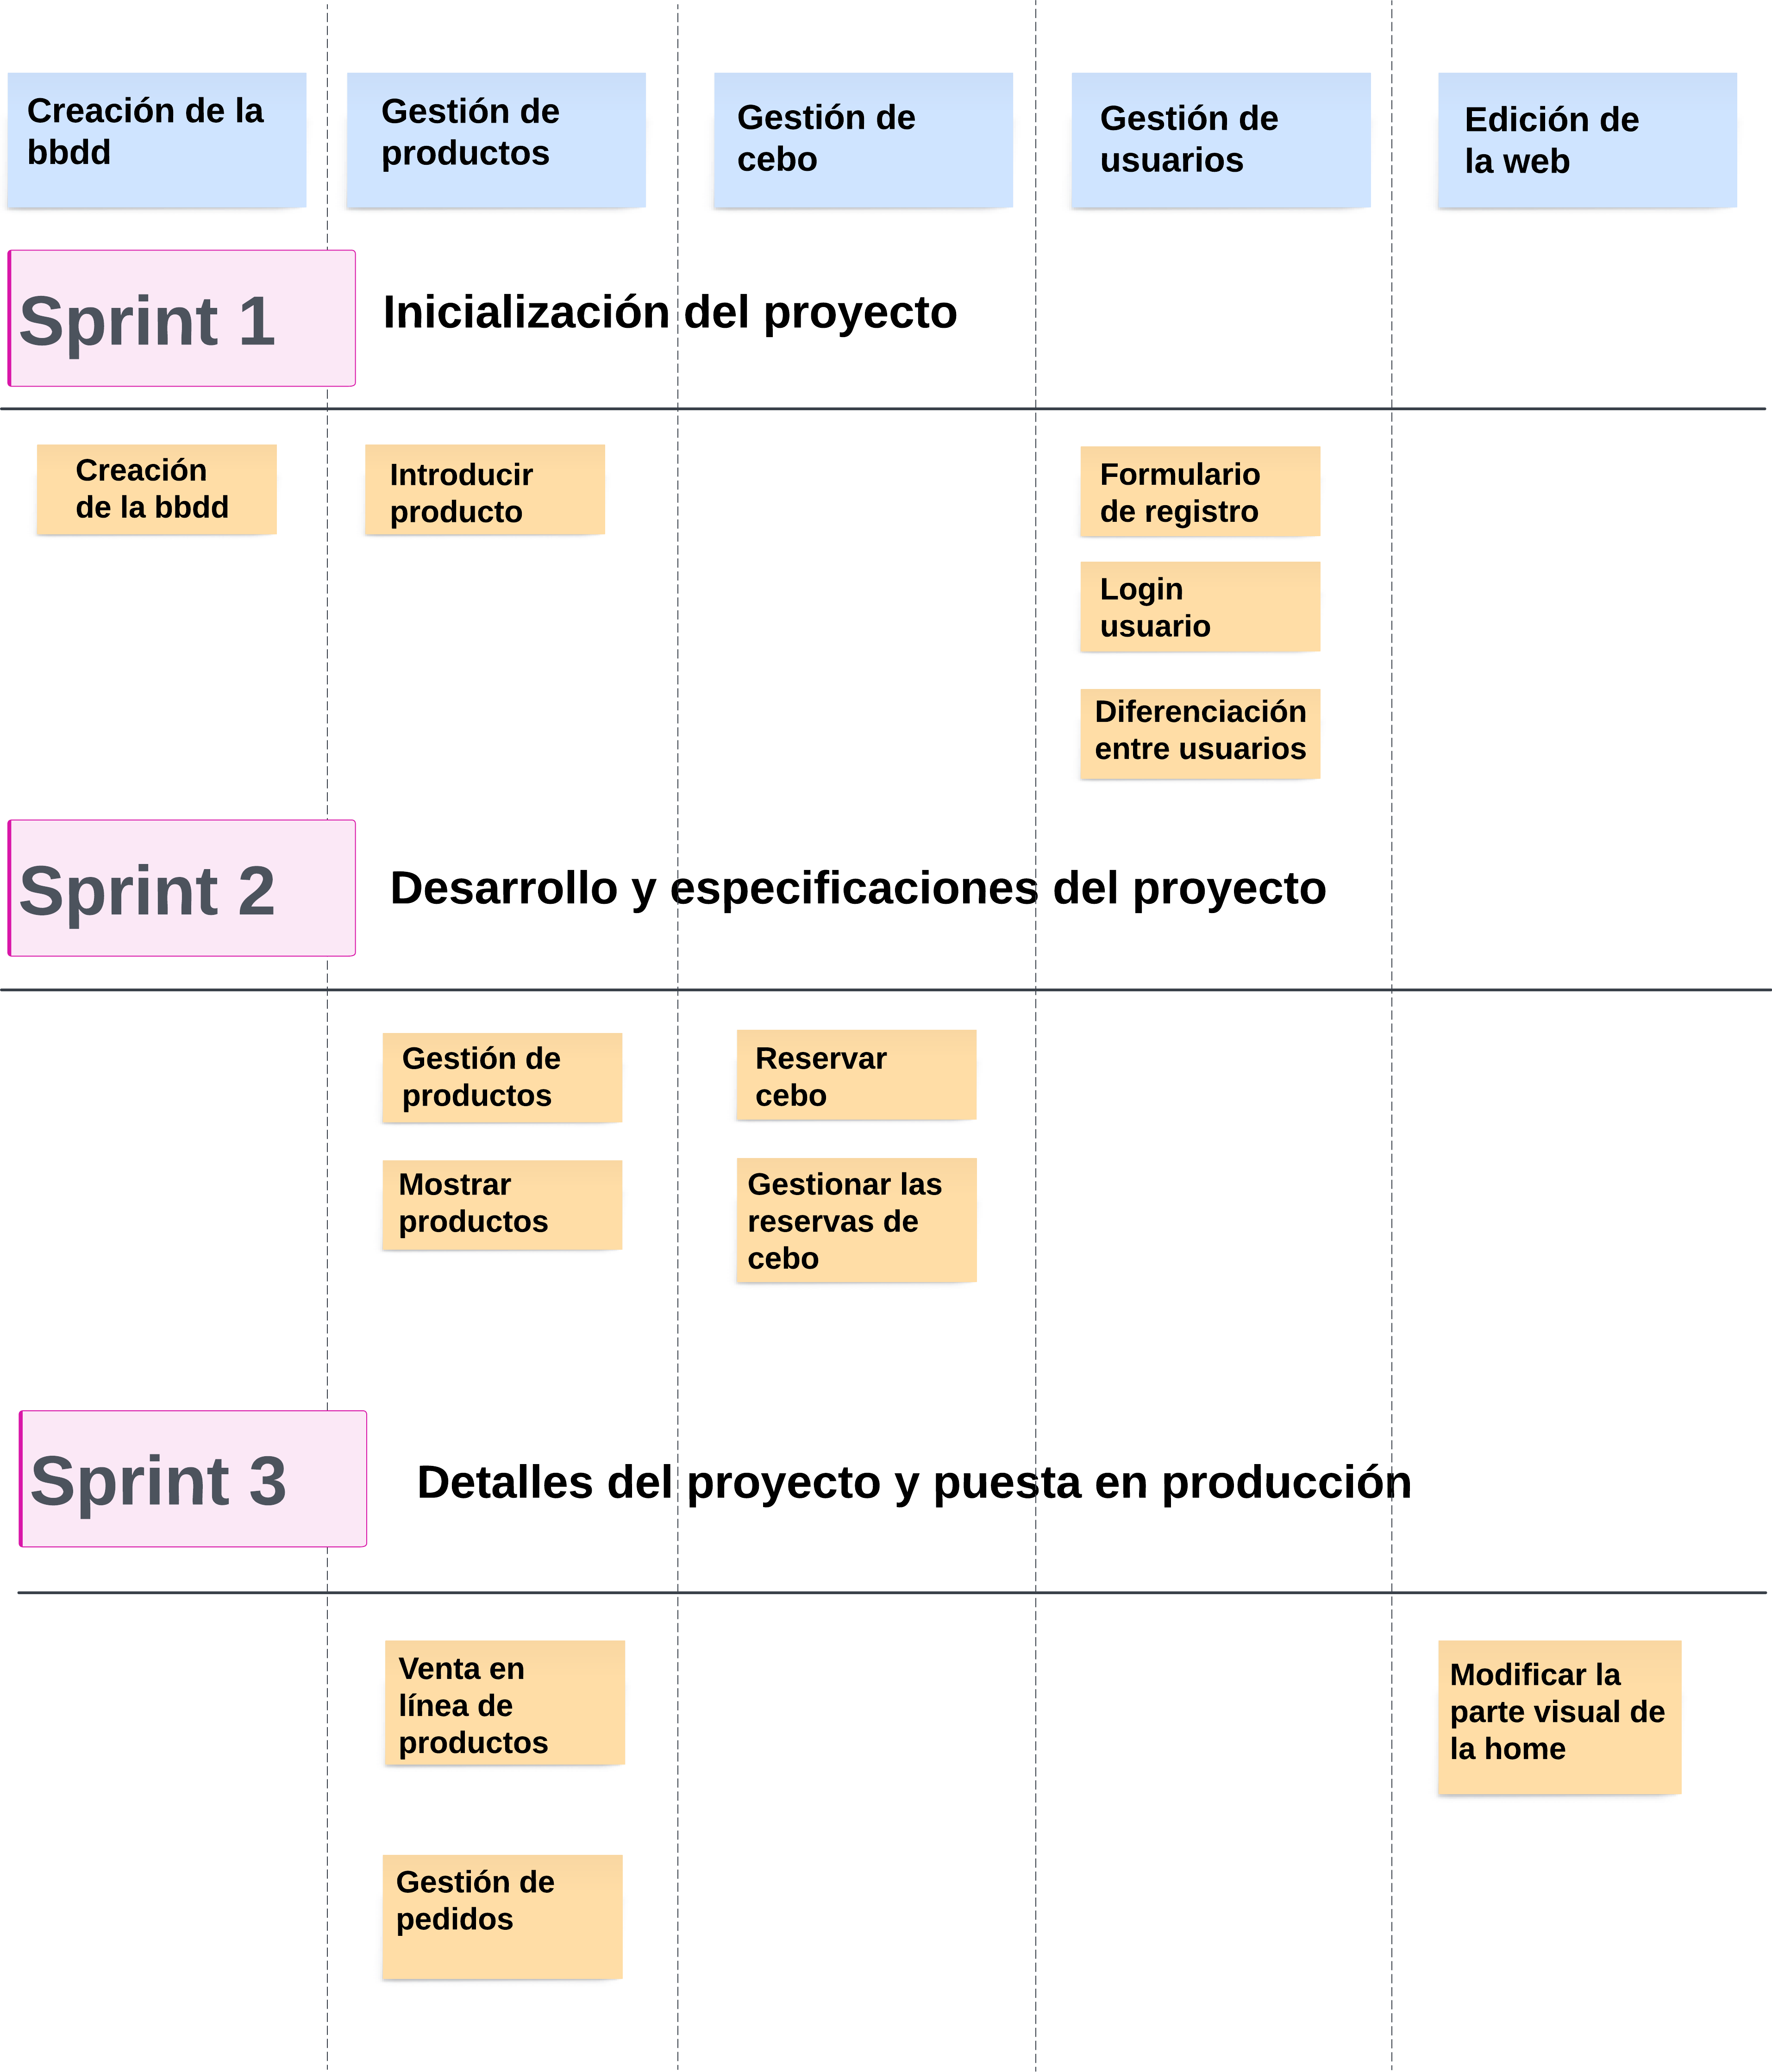
\includegraphics[scale=0.11]{./Images/MapaHistoriasUsuario.png}
\caption{Mapa de historias de usuario}

\label{fig:fig1}

\end{center}
\end{figure}

\subsection{Sprints}\label{subsec4.1.3}

A partir del mapa de historias de usuario se han generado 3 Sprints para llevar a cabo todas las tareas.

\begin{itemize}
    \item \textbf{Sprint 1: }Se comenzará con la creación de la base de datos, la funcionalidad para introducir un producto y la implementación del registro de usuarios. Además, se desarrollará el sistema de login y se diferenciarán los roles de usuario, especialmente entre administrador y usuarios regulares.

    \item \textbf{Sprint 2: }Se procederá con la gestión de productos, la funcionalidad para mostrar productos organizados por categorías y el sistema de reservas de cebo. También se implementará la gestión de las reservas de cebo por parte del administrador, garantizando que estén listas para la fecha de recogida.
    
    \item \textbf{Sprint 3: }Se desarrollará la venta en línea de productos, incluyendo la adición de productos al carrito y la gestión de pedidos. Además, se implementará la funcionalidad para modificar la parte visual de la página de inicio (home).
    
\end{itemize}

\section{Modelos para la interfaz - Mockup}\label{sec:apartado}
En este apartado, nos adentraremos en el proceso de diseño de la interfaz de usuario para nuestra aplicación. La interfaz de usuario desempeña un papel crucial en la experiencia del usuario, ya que actúa como el punto de interacción principal entre los usuarios y la funcionalidad ofrecida por la aplicación. Para garantizar una experiencia de usuario intuitiva y atractiva, es fundamental desarrollar una interfaz bien diseñada que refleje las necesidades y expectativas de nuestros usuarios.

\vspace{0.5cm}

Para alcanzar este objetivo, hemos empleado una metodología centrada en el usuario que comienza con la creación de modelos para la interfaz, conocidos como mockups. Estos mockups proporcionan representaciones visuales de la estructura y el diseño de la interfaz para diferentes tipos de usuarios, incluidos clientes y administradores. Además de las vistas de cliente y administrador, hemos agregado la vista de registro de usuario y login. Es importante destacar que el proceso de login será el mismo tanto para los clientes como para los administradores, proporcionando una experiencia unificada para todos los usuarios. En la vista del cliente, nos enfocaremos en proporcionar una experiencia de compra fluida y agradable, mientras que en la vista del administrador nos concentraremos en herramientas de gestión y control para administrar eficientemente la plataforma.

\subsection{Mockup registro y login}\label{subsec4.2.1}

En la Figura 4.2 se muestra la pantalla de registro de usuarios. Esta interfaz permite a los usuarios crear una cuenta en nuestra plataforma proporcionando la información necesaria de manera clara y sencilla.

\begin{figure}[H]
\begin{center}
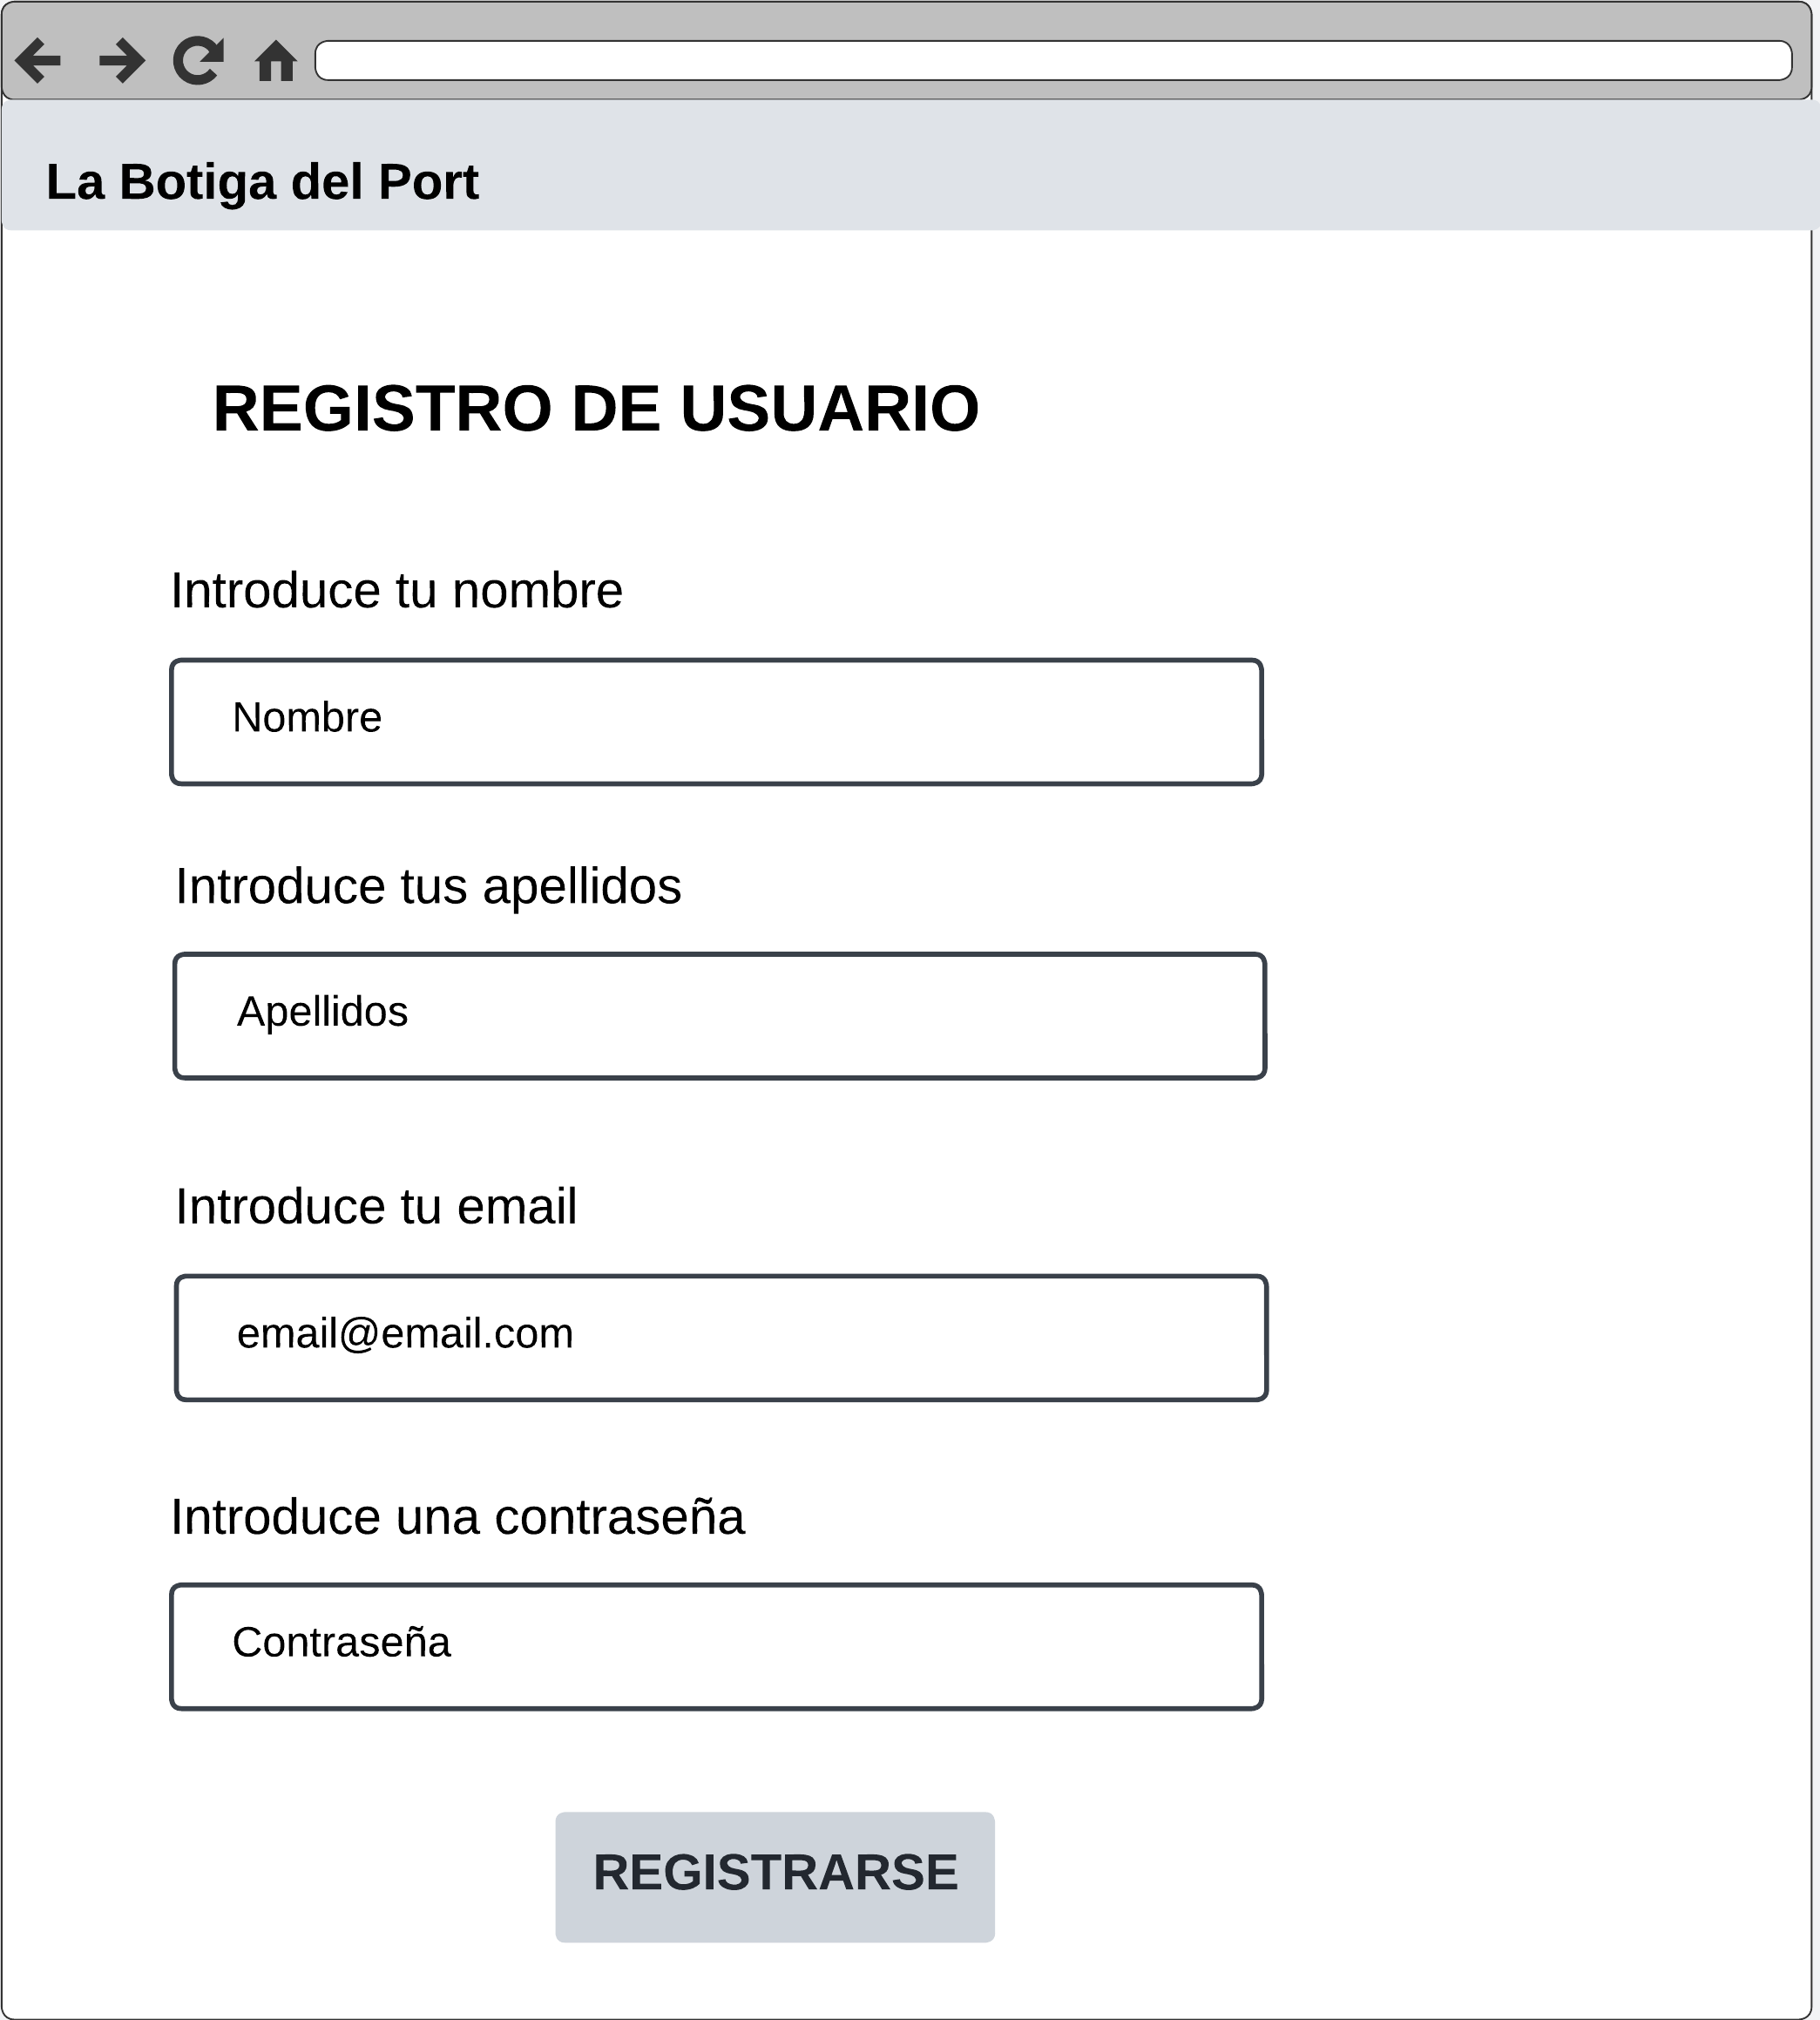
\includegraphics[scale=0.5]{./Images/registro.png}
\caption{Modelo de registro.} Fuente: Elaboración propia.

\label{fig:fig2}

\end{center}
\end{figure}


La Figura 4.3 presenta la pantalla de inicio de sesión. Aquí, los usuarios pueden acceder a sus cuentas ingresando su correo electrónico y contraseña de forma segura.


\begin{figure}[H]
\begin{center}
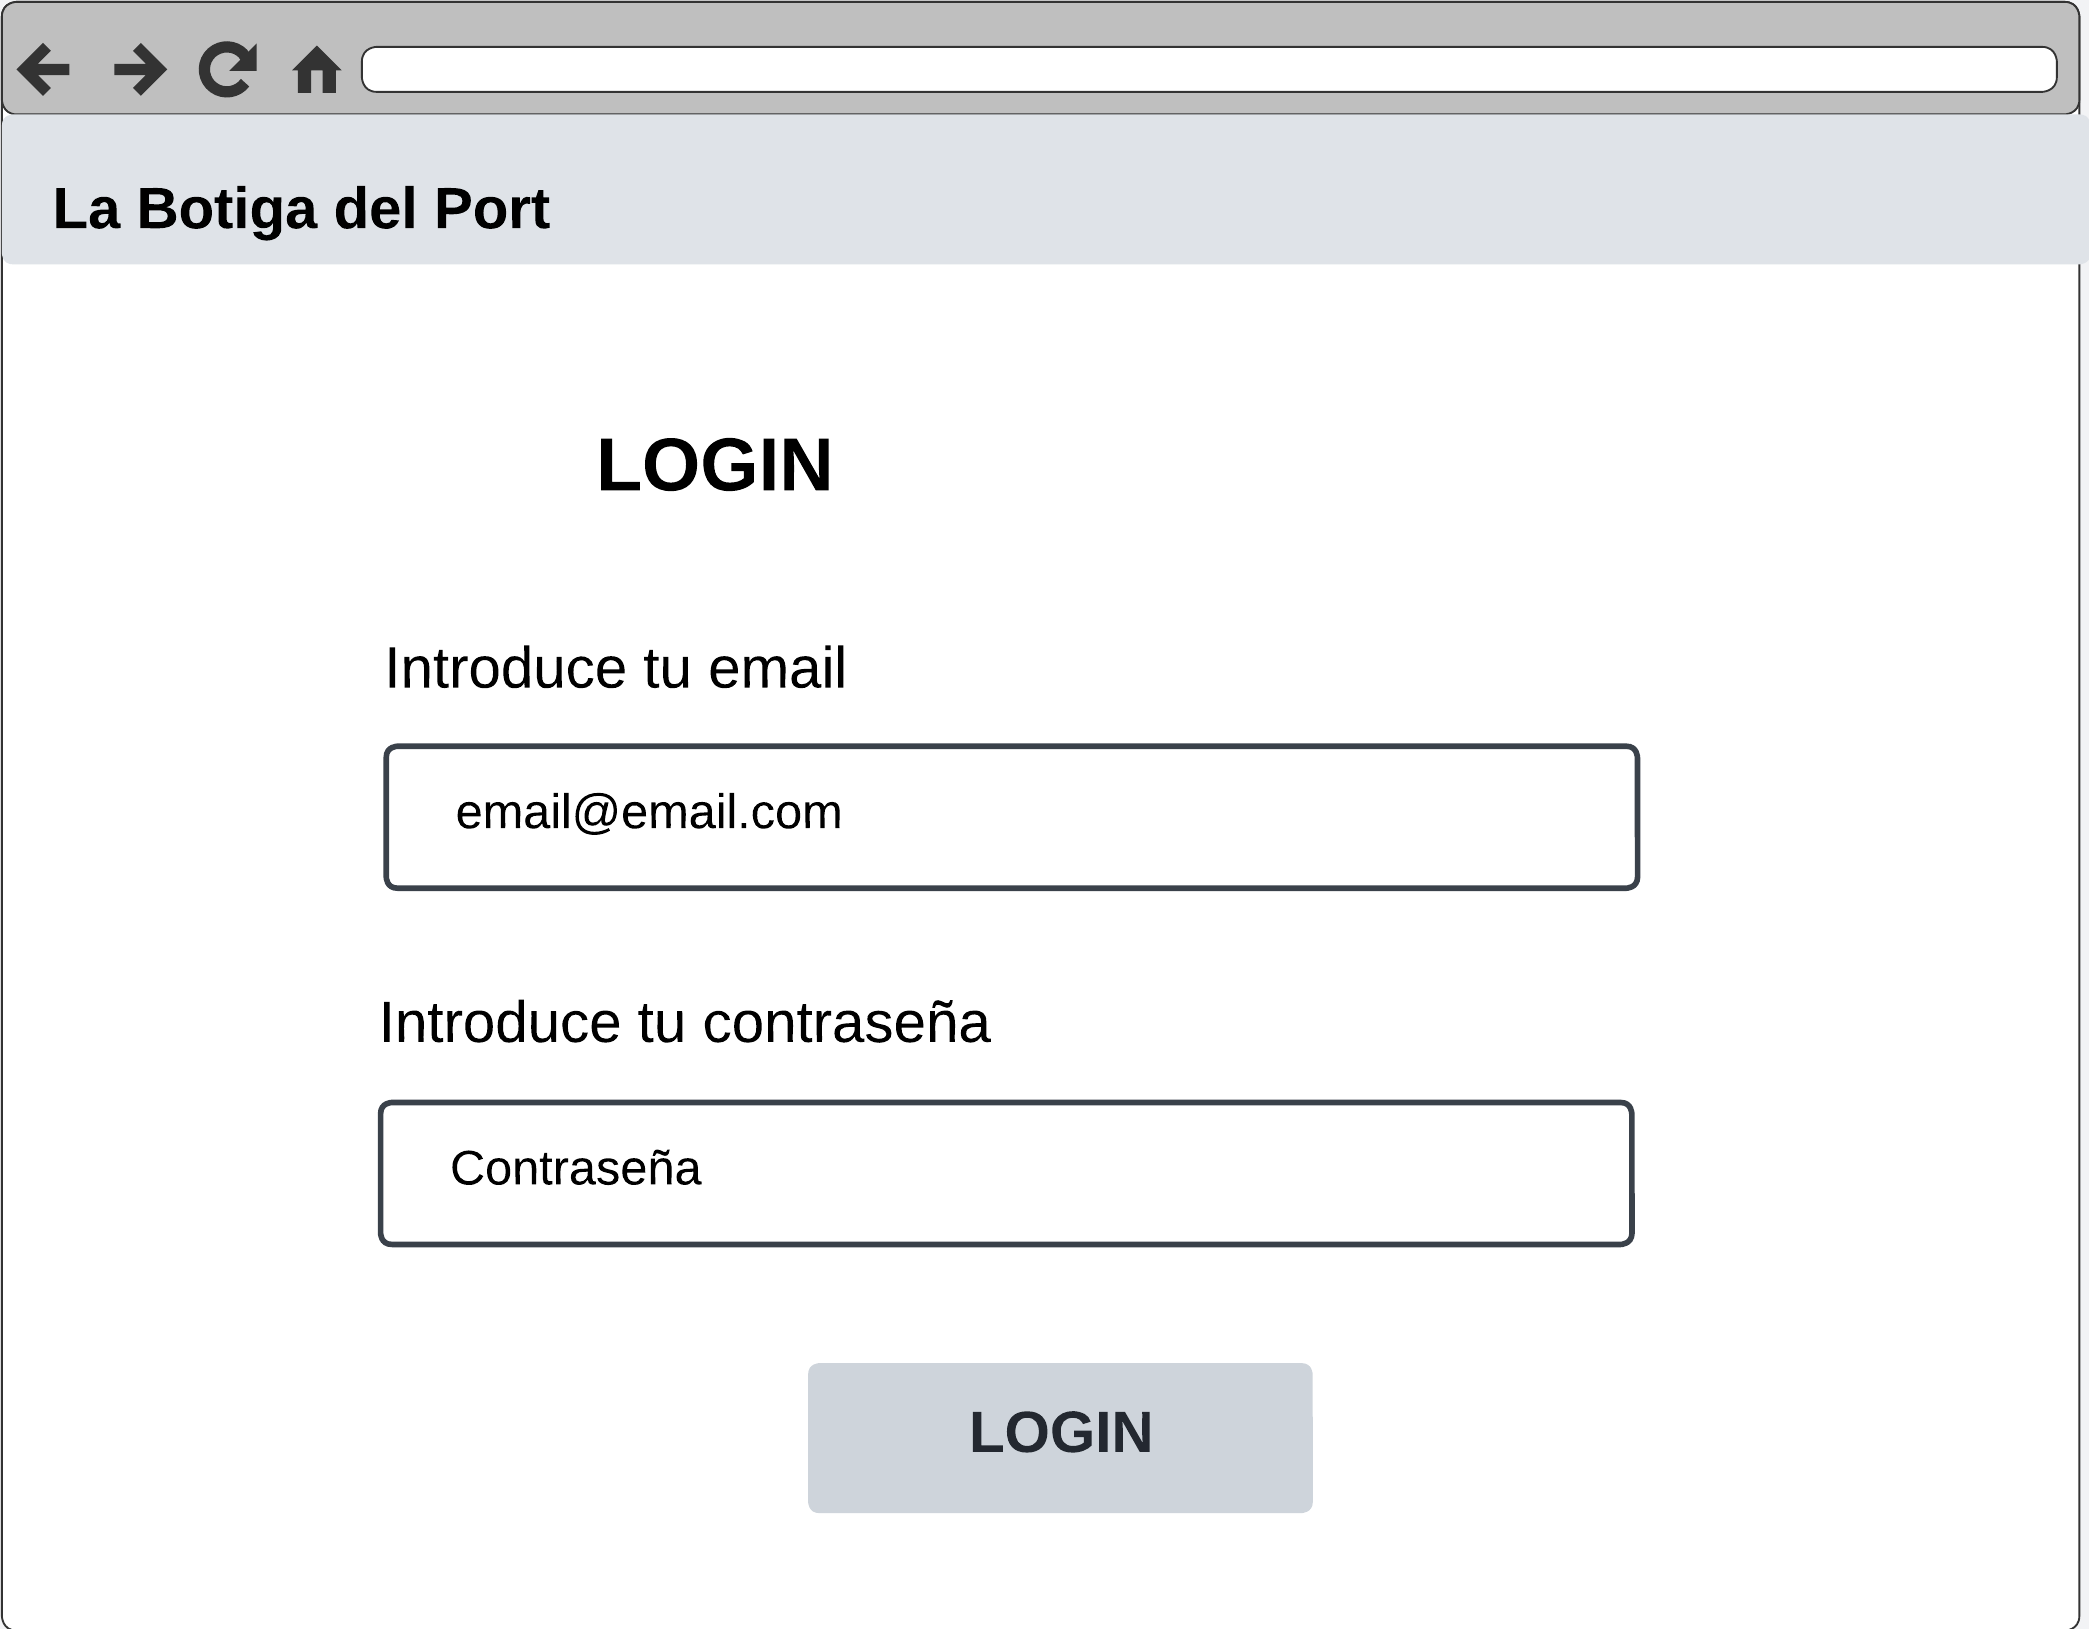
\includegraphics[scale=0.5]{./Images/login.png}
\caption{Modelo de Login.} Fuente: Elaboración propia.

\label{fig:fig3}

\end{center}
\end{figure}

\subsection{Mockup para el cliente}\label{subsec4.2.2}

La Figura 4.4 muestra una de las páginas principales de productos de nuestra aplicación. En esta vista, los usuarios pueden explorar una selección de productos y acceder al detale de cada uno de los productos. 

\begin{figure}[H]
\begin{center}
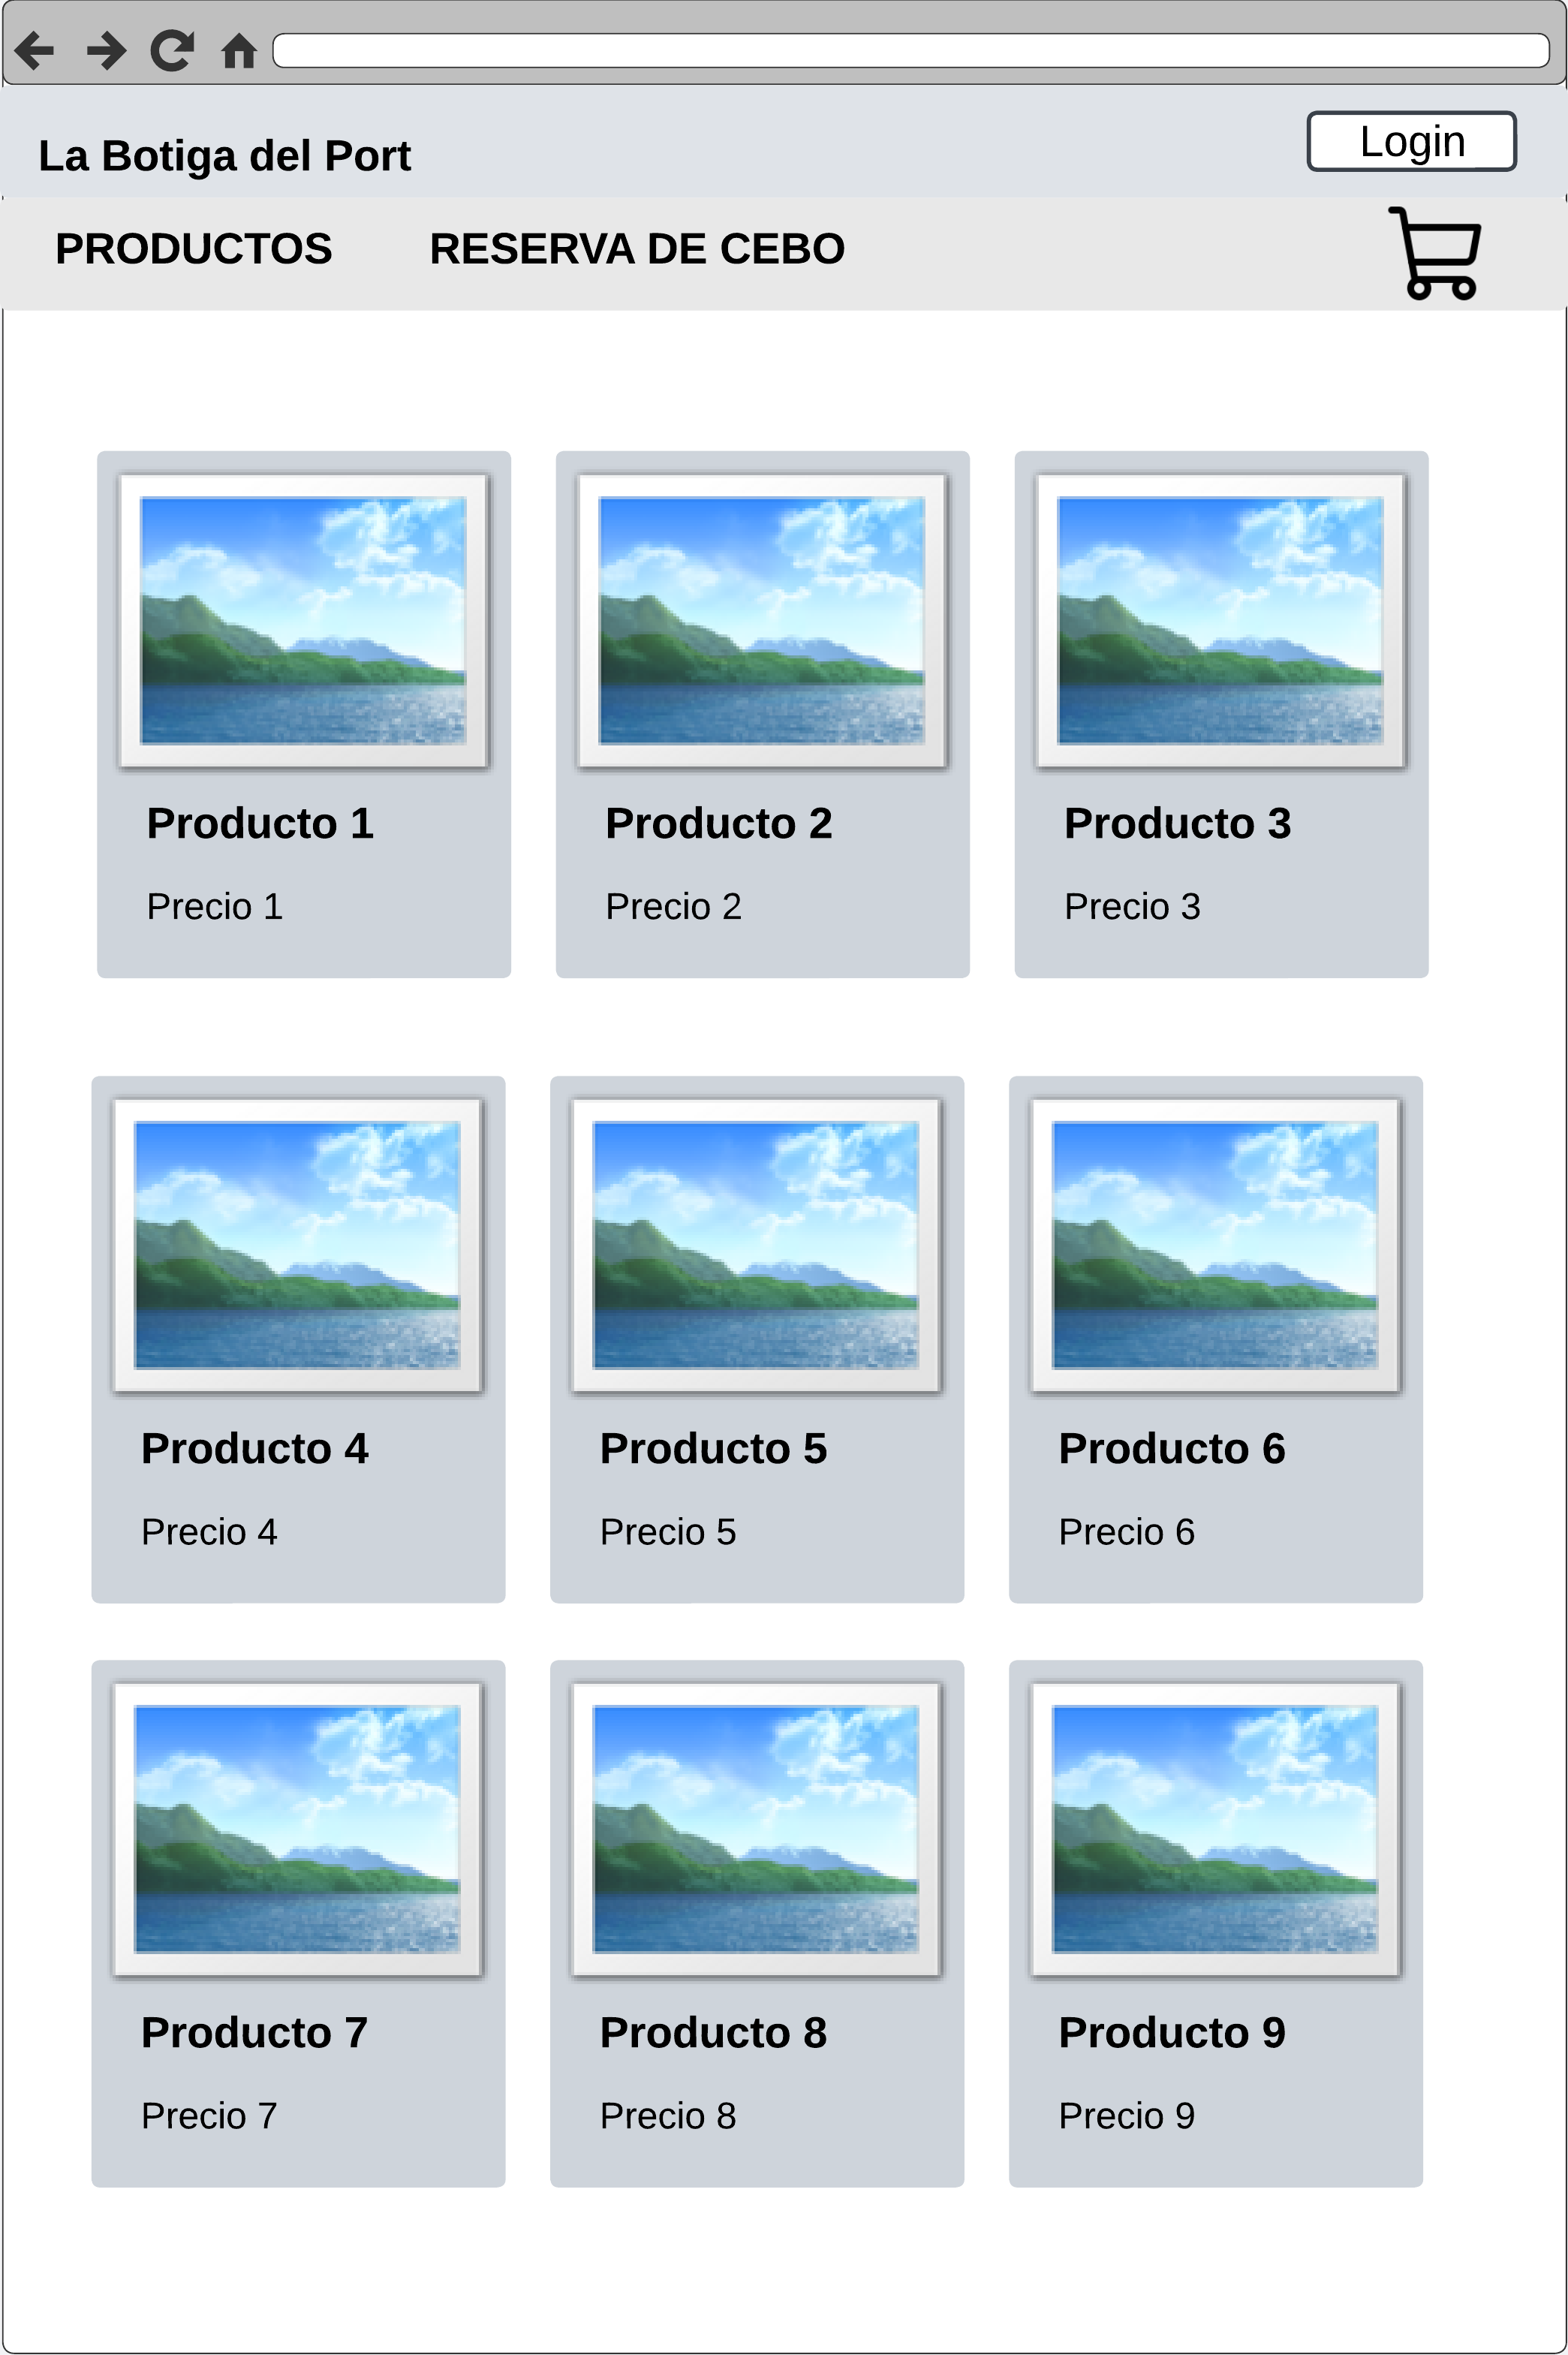
\includegraphics[scale=0.5]{./Images/productos.png}
\caption{Modelo de cliente - Página de productos.} Fuente: Elaboración propia.

\label{fig:fig4}

\end{center}
\end{figure}

En la Figura 4.5 se presenta el detalle del producto. Esta interfaz proporciona a los usuarios información detallada sobre un producto específico, incluyendo su descripción, precio y opciones de compra. 

\begin{figure}[H]
\begin{center}
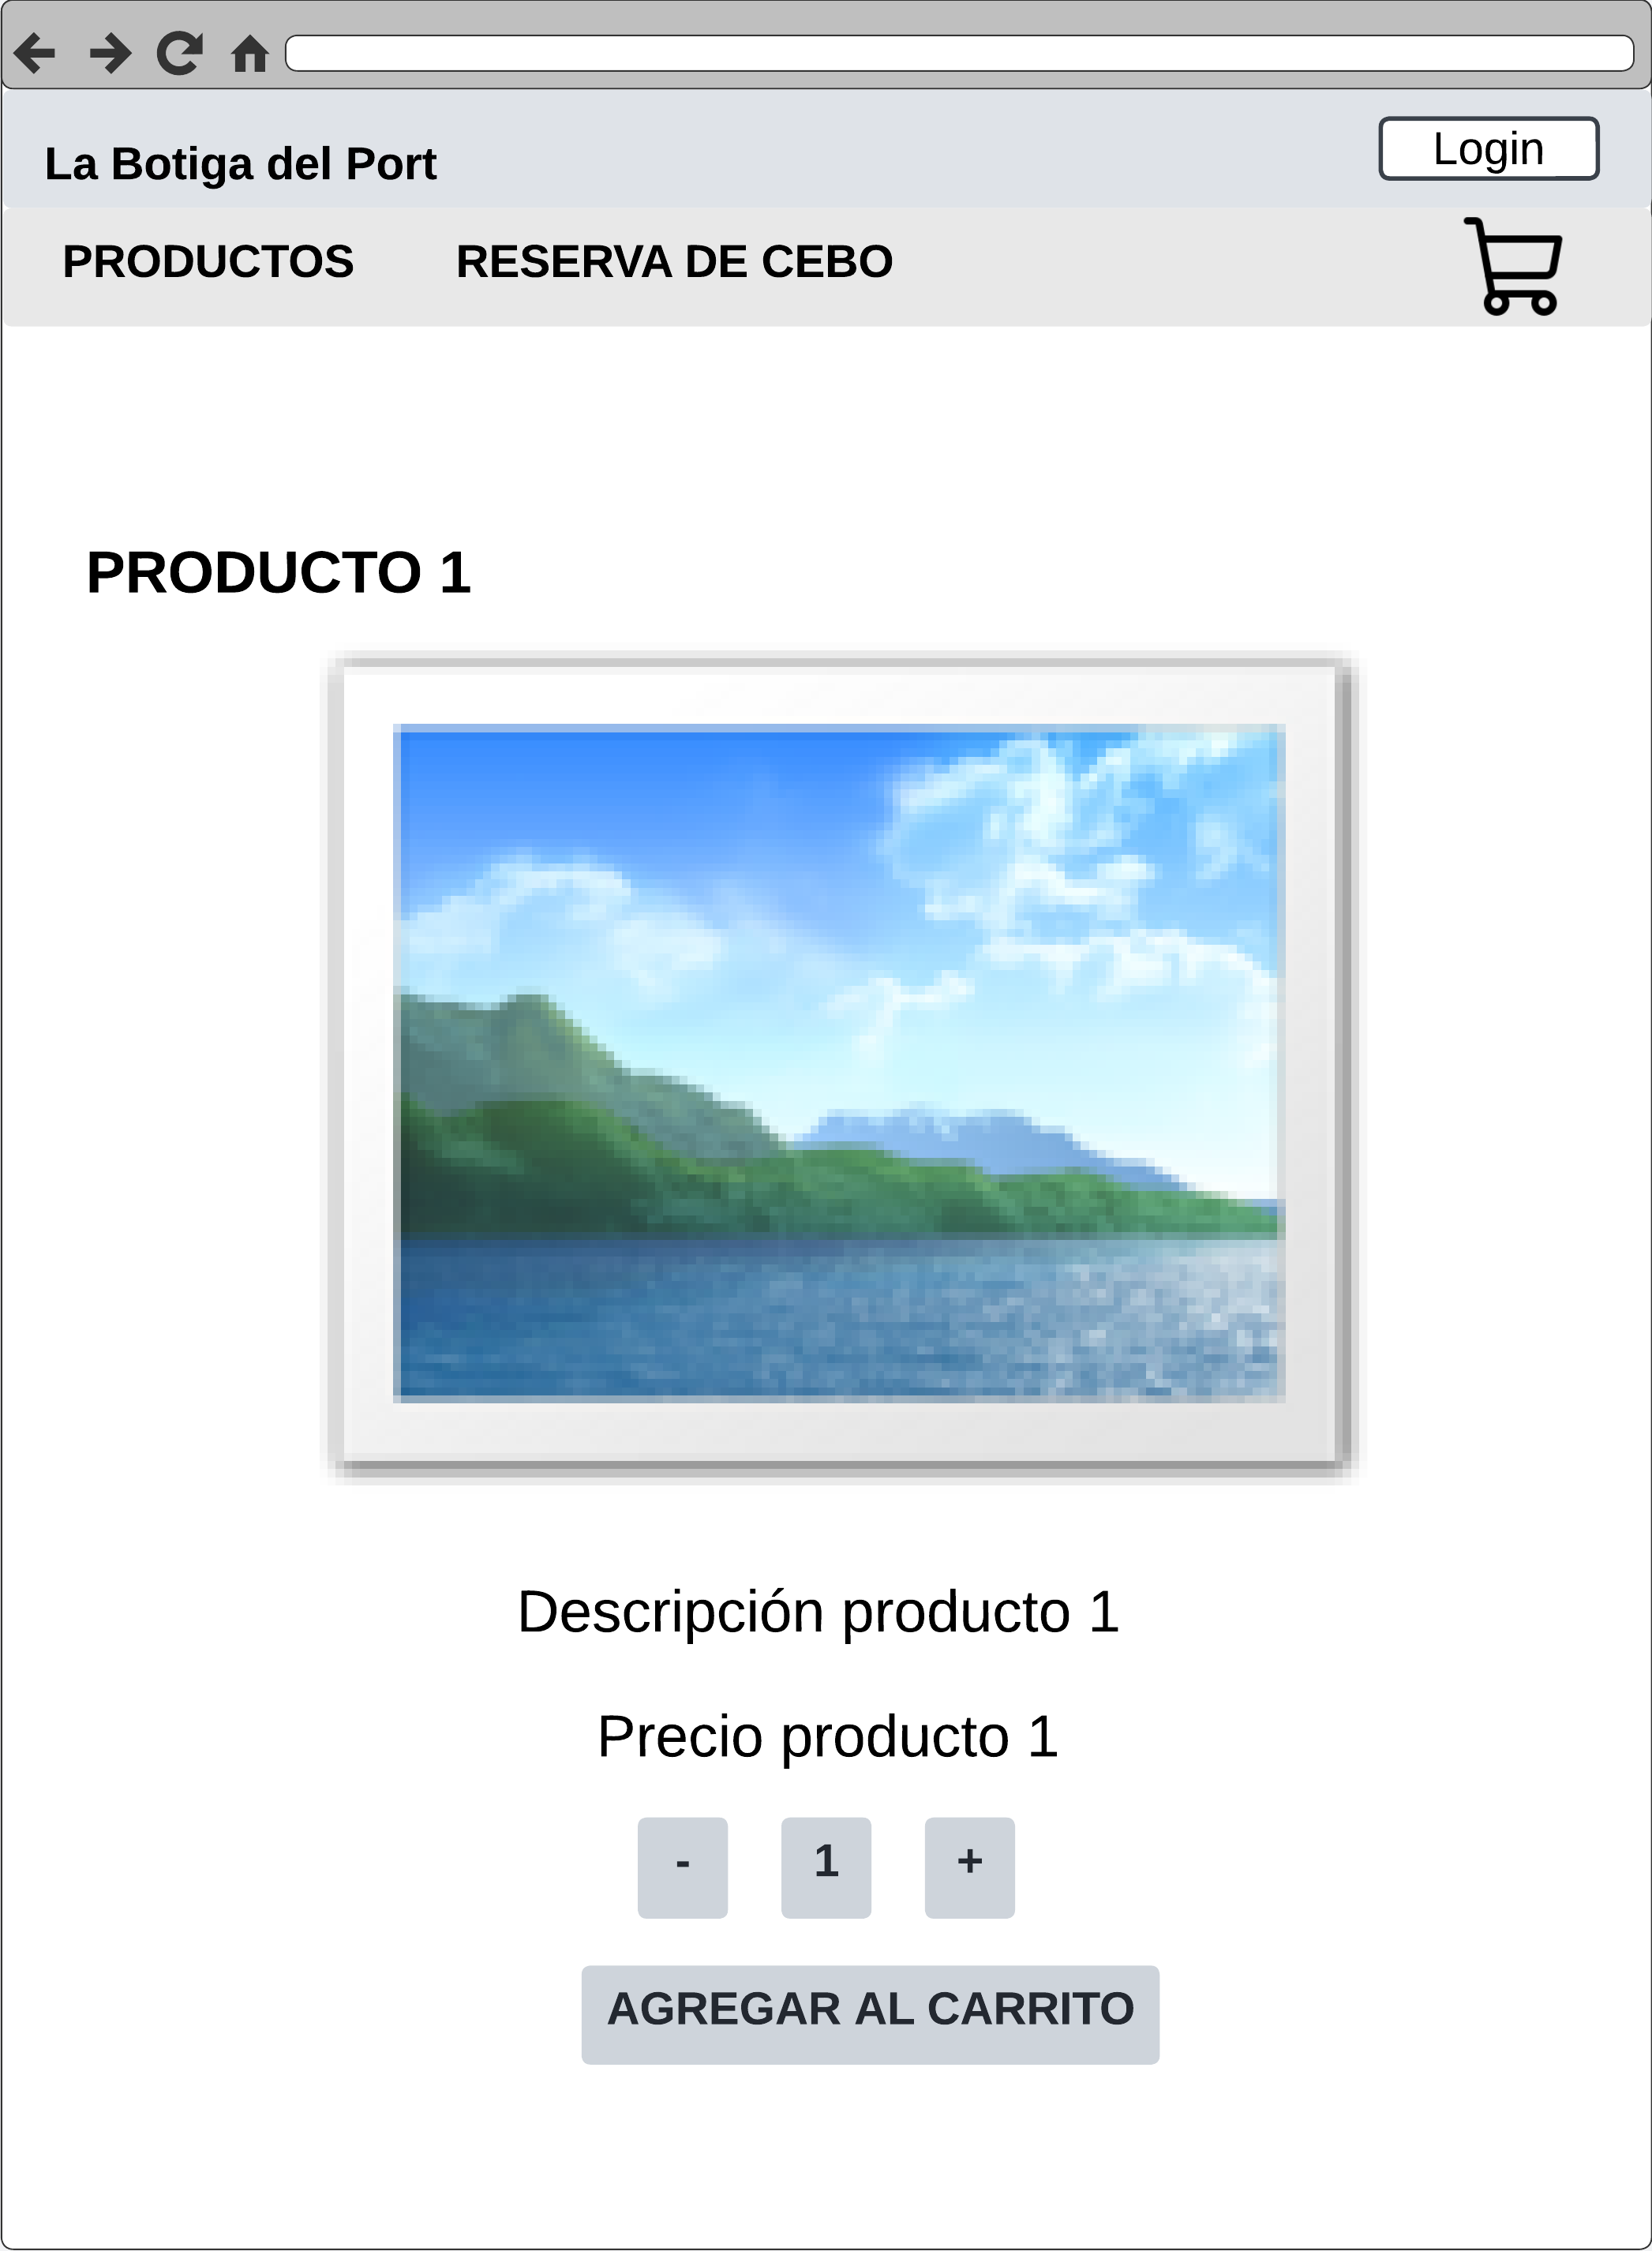
\includegraphics[scale=0.5]{./Images/detalle_producto.png}
\caption{Modelo de cliente - Página detalle del producto.} Fuente: Elaboración propia.

\label{fig:fig5}

\end{center}
\end{figure}

La Figura 4.6 muestra el resumen del pedido. Aquí, los usuarios pueden revisar y confirmar los productos seleccionados antes de finalizar su compra.


\begin{figure}[H]
\begin{center}
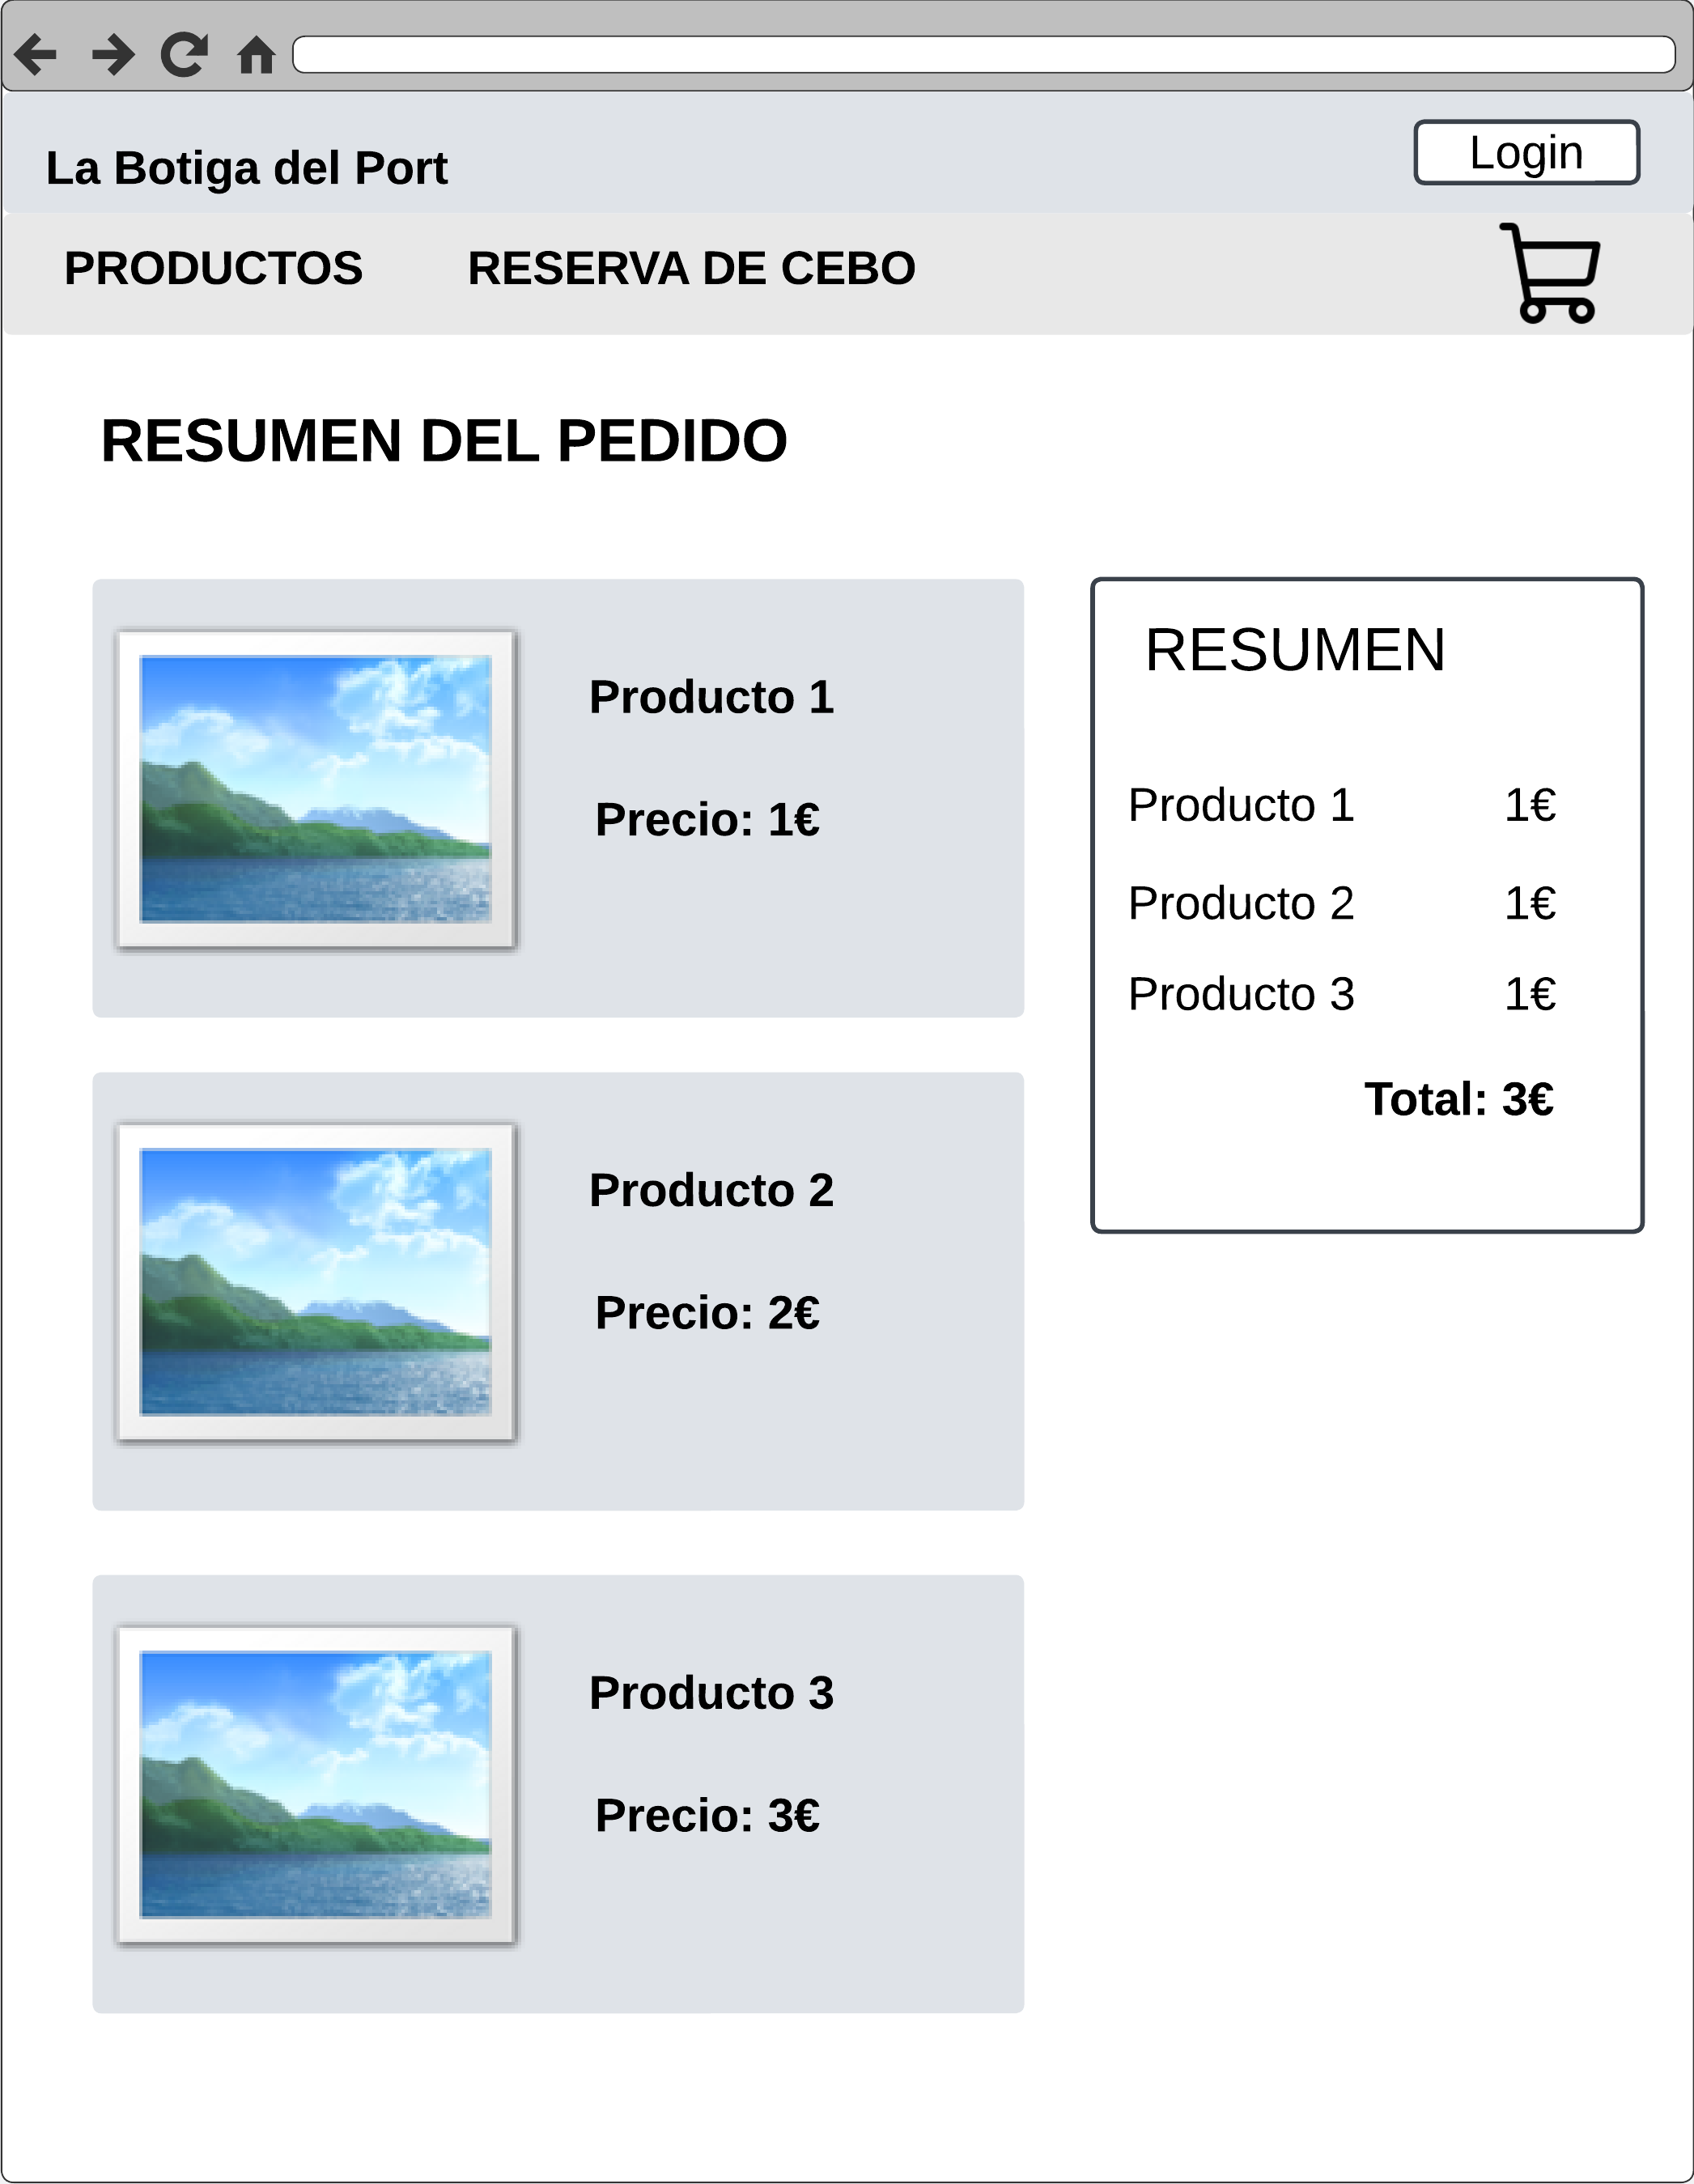
\includegraphics[scale=0.5]{./Images/pedido.png}
\caption{Modelo de cliente - Resumen del pedido.} Fuente: Elaboración propia.

\label{fig:fig6}

\end{center}
\end{figure}

En la Figura 4.7 se presenta la interfaz de reserva de cebo. Esta función permite a los usuarios reservar cebo disponible en la tienda para su compra posterior, asegurando que el cebo deseado esté reservado y disponible cuando el usuario lo necesite.


\begin{figure}[H]
\begin{center}
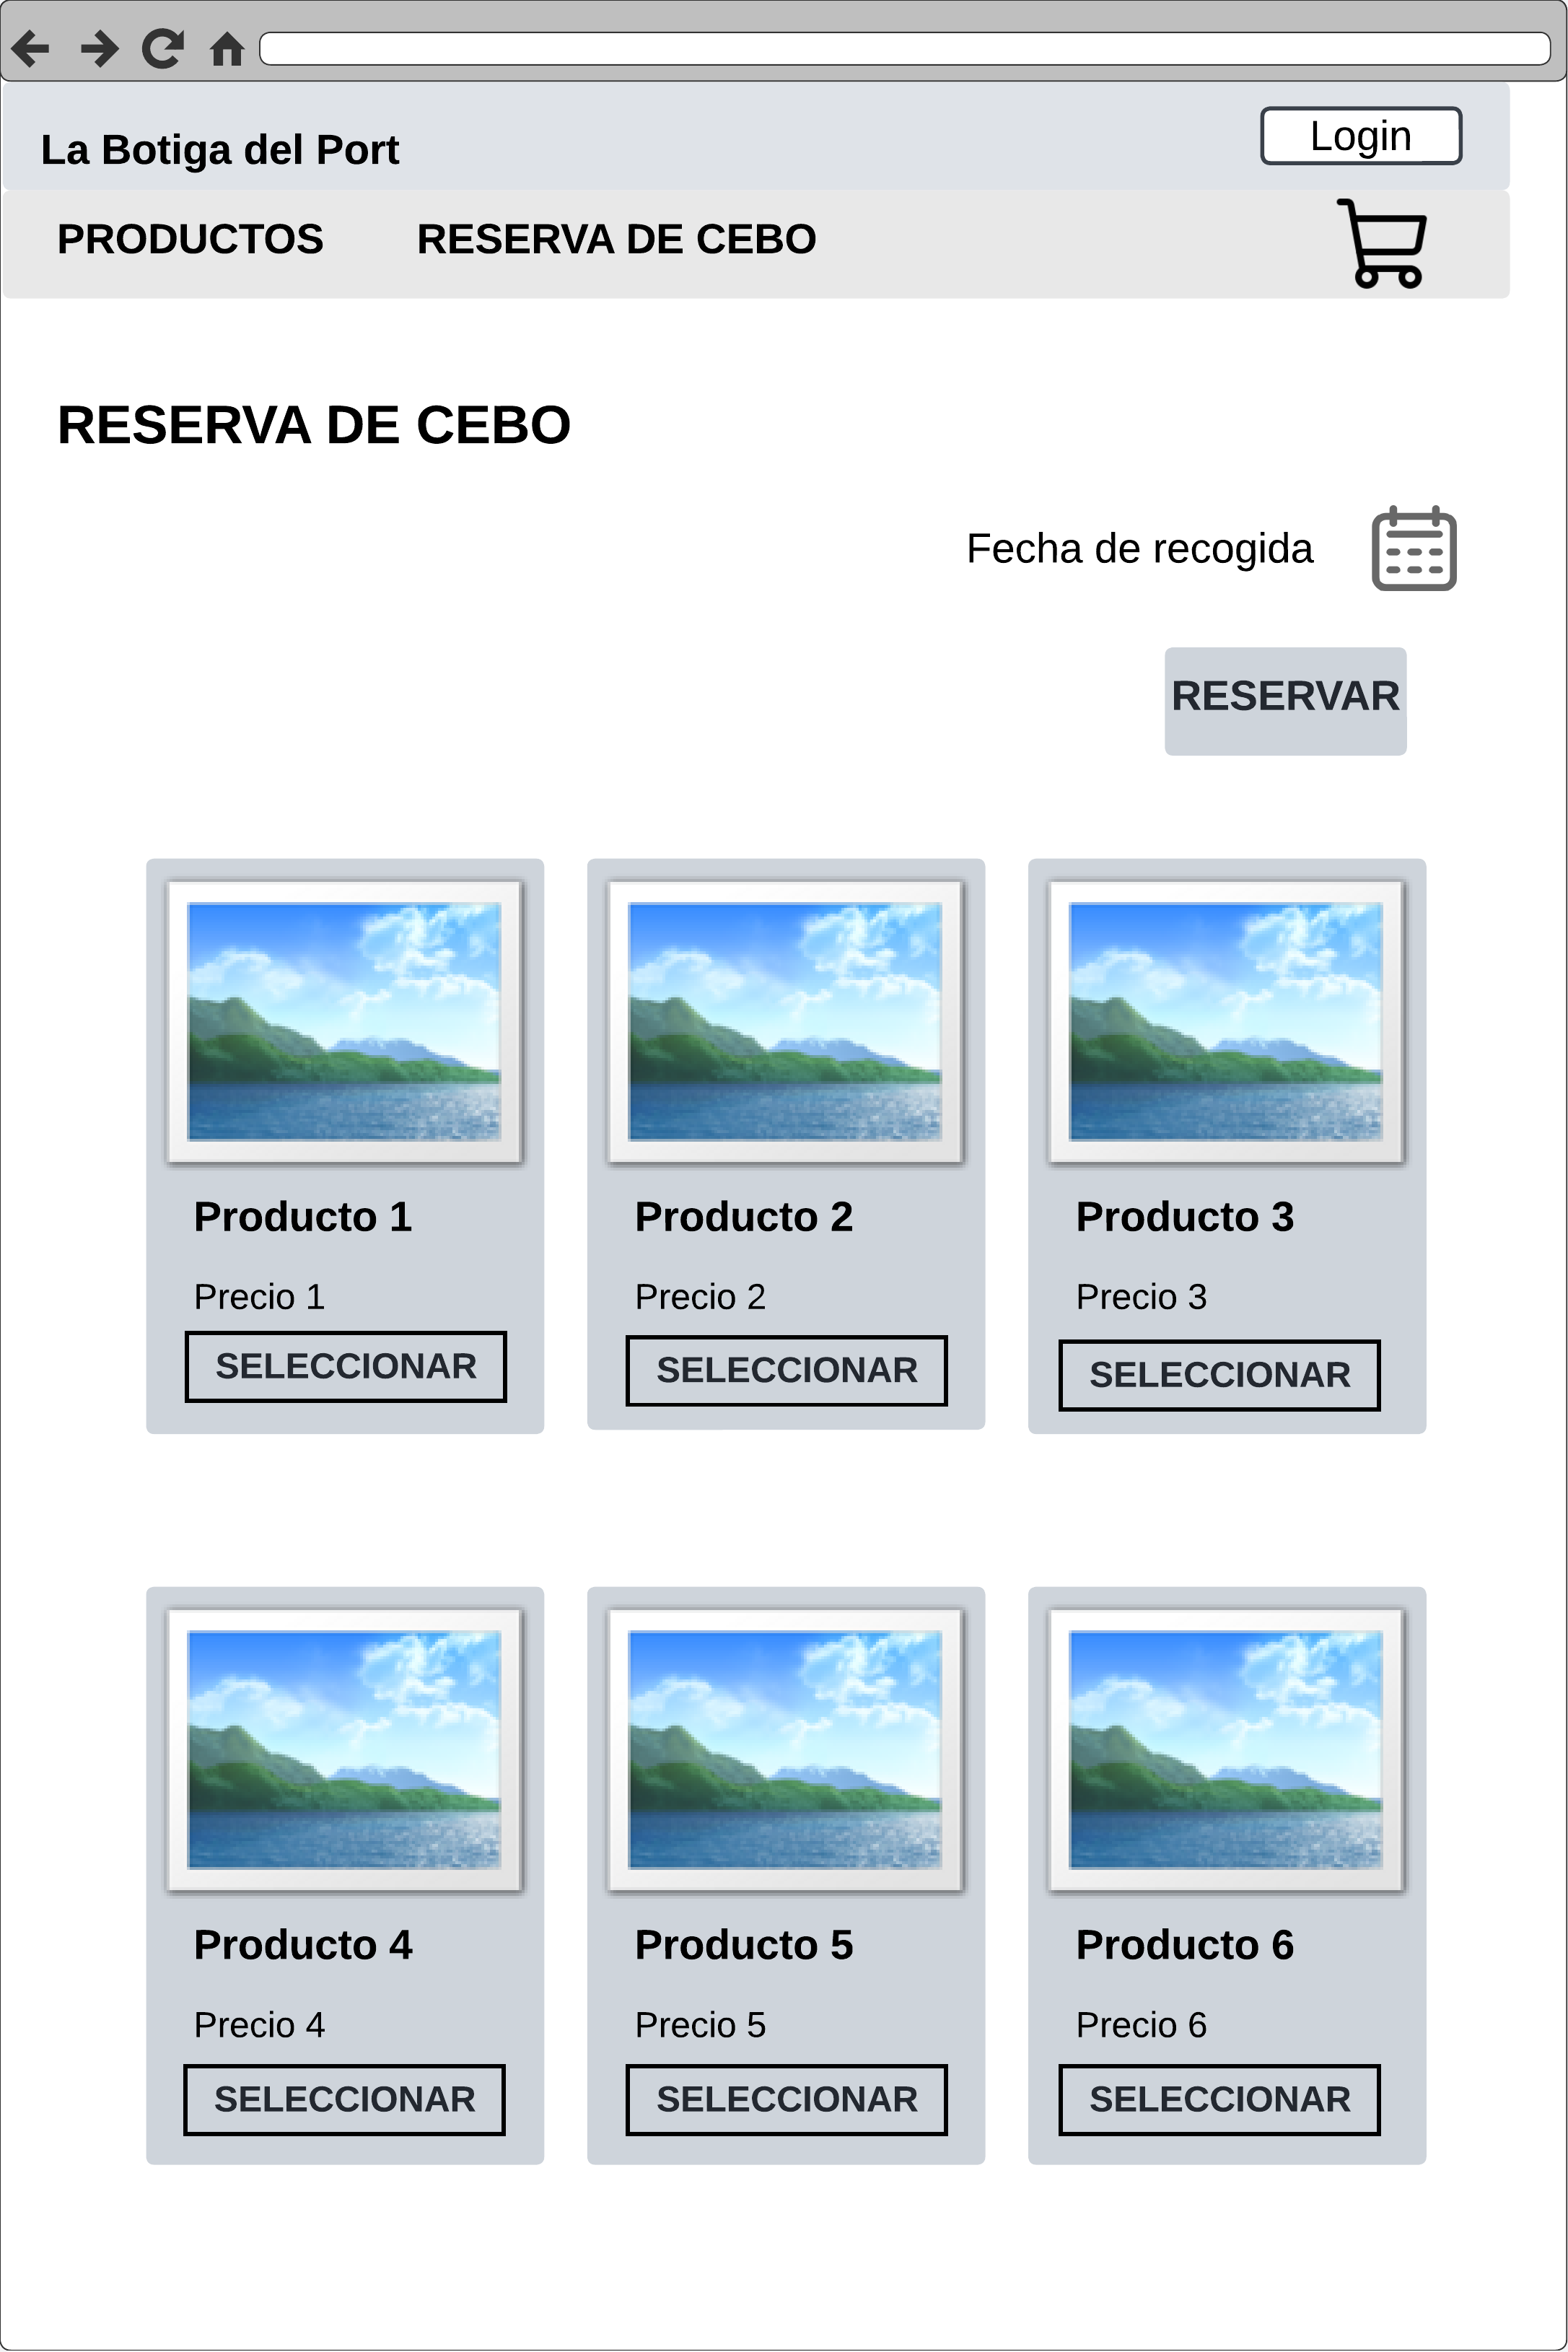
\includegraphics[scale=0.5]{./Images/reserva_cebo.png}
\caption{Modelo de cliente - Reserva de cebo.} Fuente: Elaboración propia.

\label{fig:fig7}

\end{center}
\end{figure}

\subsection{Mockup para el administrador}\label{subsec4.2.3}

En la Figura 4.8 se presenta el formulario de nuevo producto diseñado para el modo administrador. Esta interfaz permite al administrador agregar un nuevo producto al sistema proporcionando información detallada, como nombre, descripción, precio, cantidad e imágenes, facilitando la gestión eficiente del inventario.



\begin{figure}[H]
\begin{center}
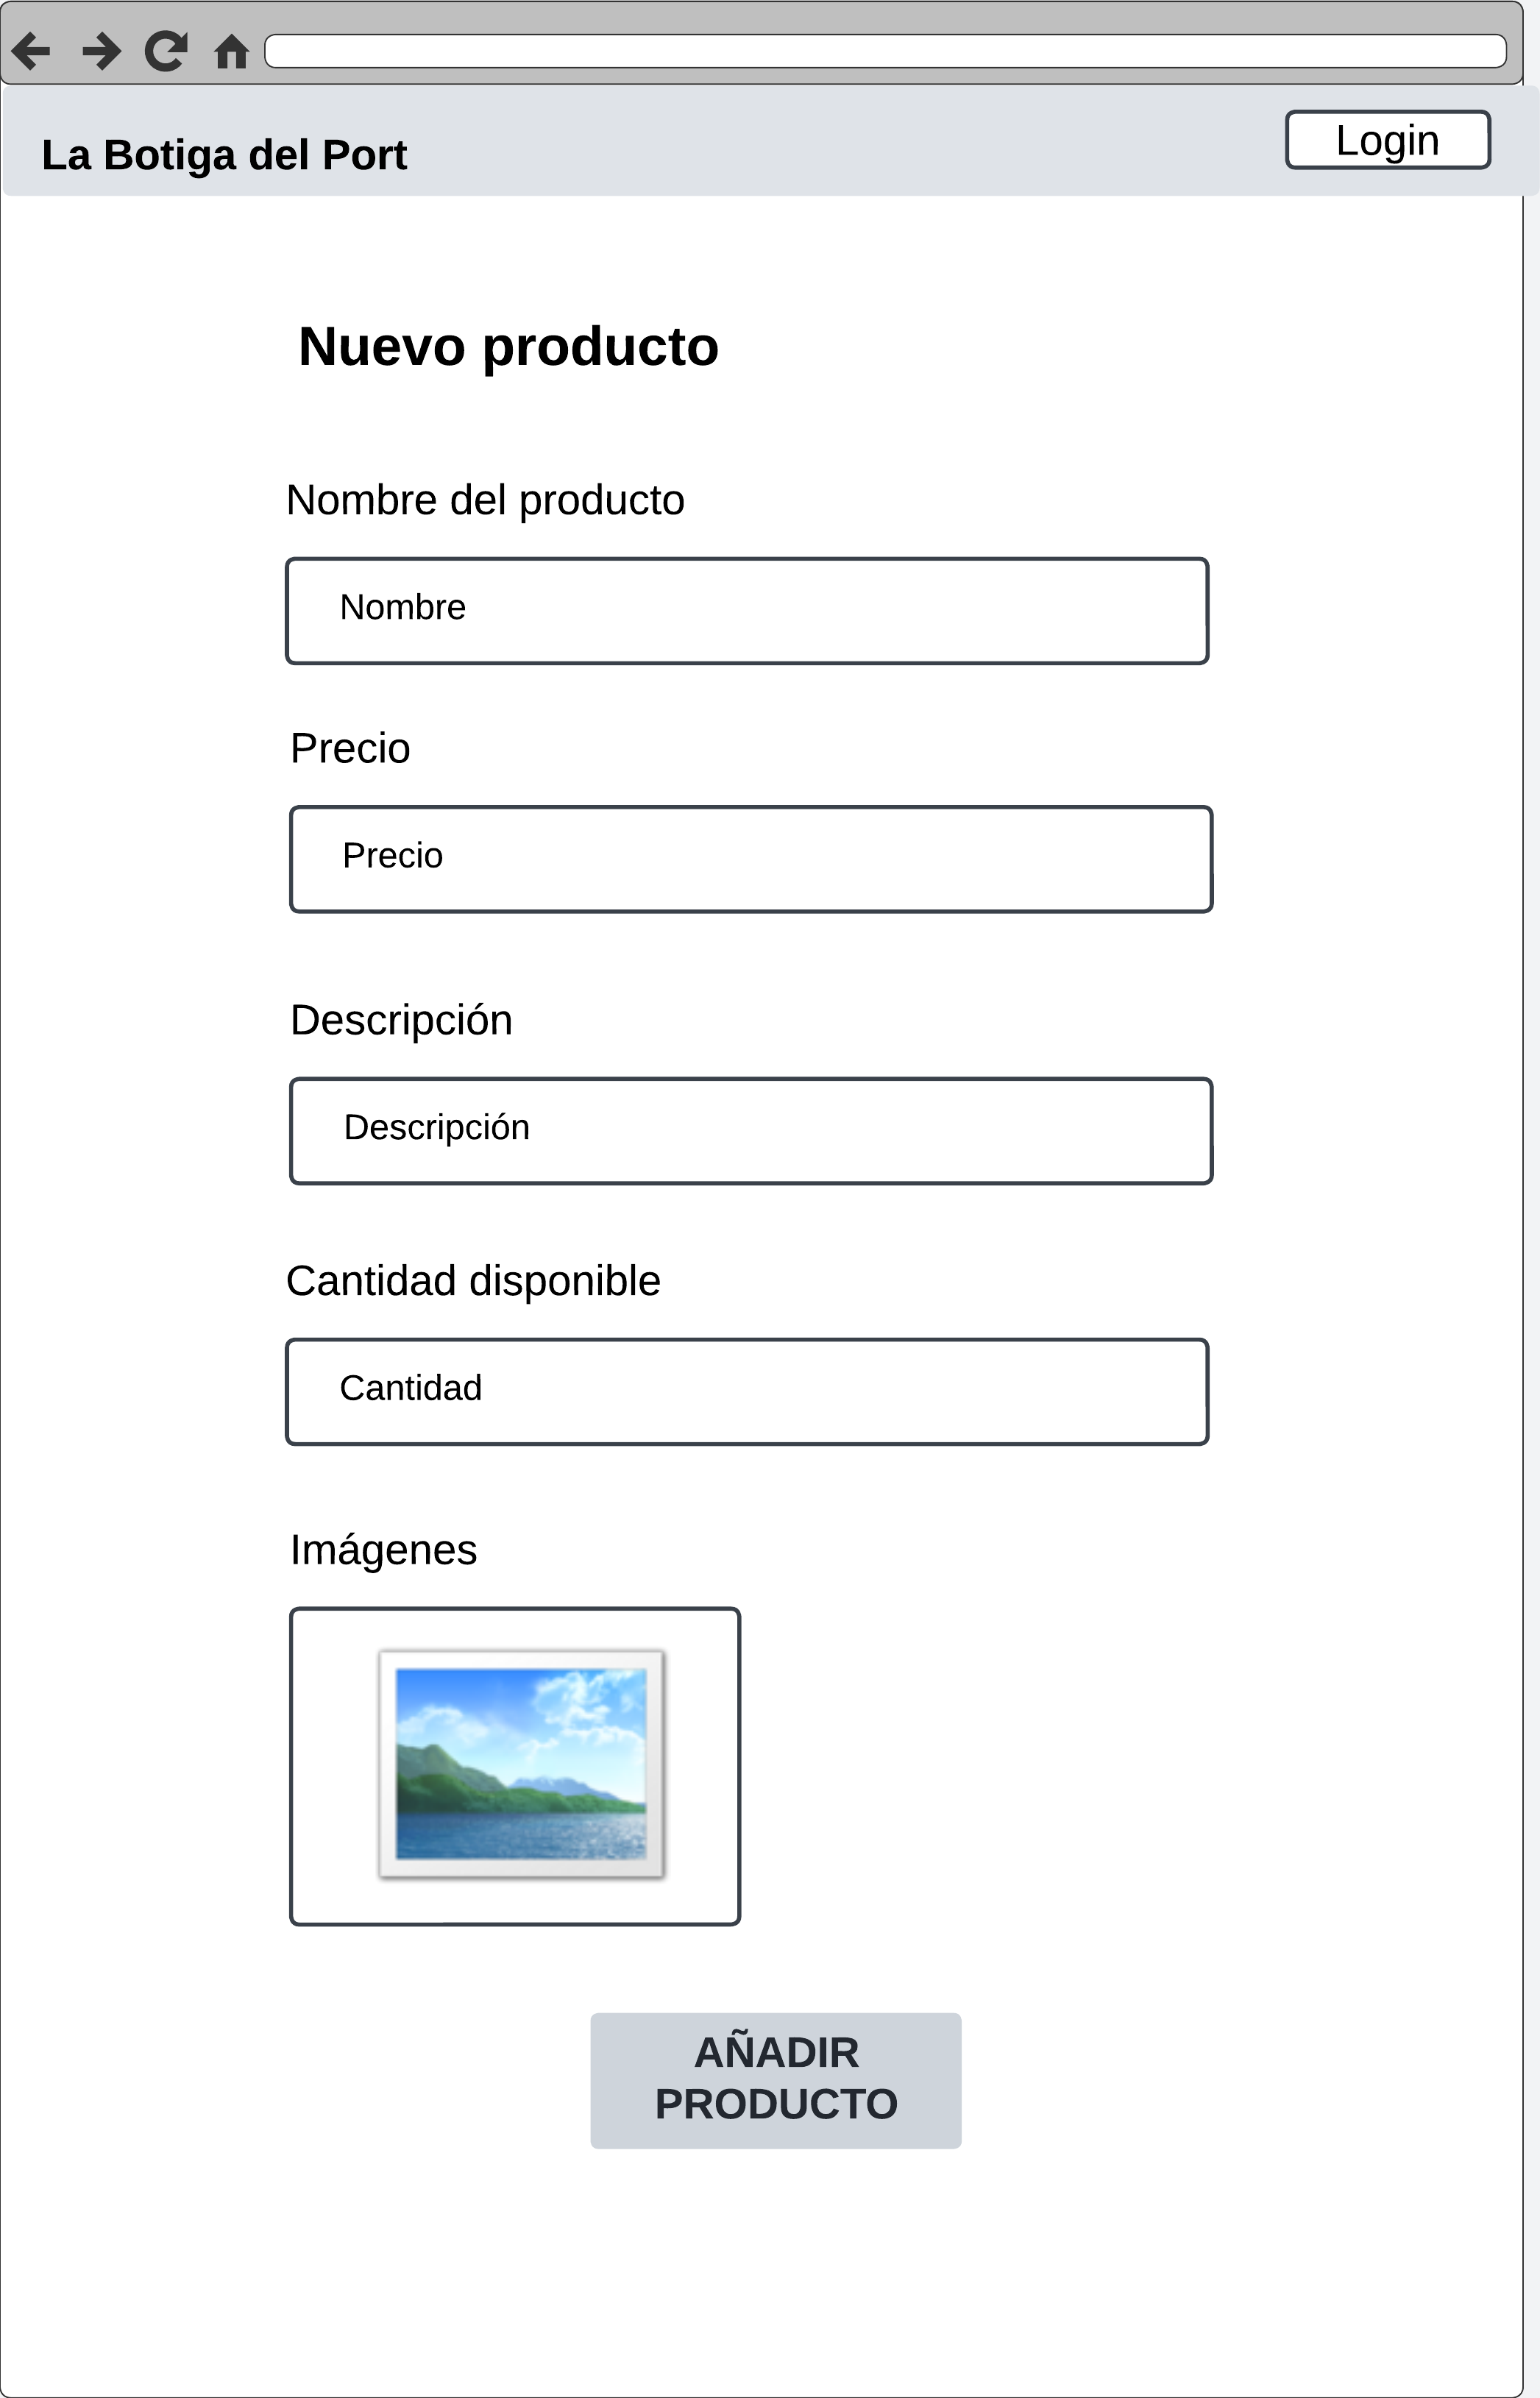
\includegraphics[scale=0.5]{./Images/nuevo_producto.png}
\caption{Modelo de administrador - Nuevo producto.} Fuente: Elaboración propia.

\label{fig:fig8}

\end{center}
\end{figure}

La Figura 4.9 muestra la vista de todos los productos existentes en el sistema. Esta interfaz proporciona al administrador una visión general de todos los productos almacenados, junto con opciones para editar o eliminar cada producto individualmente. 


\begin{figure}[H]
\begin{center}
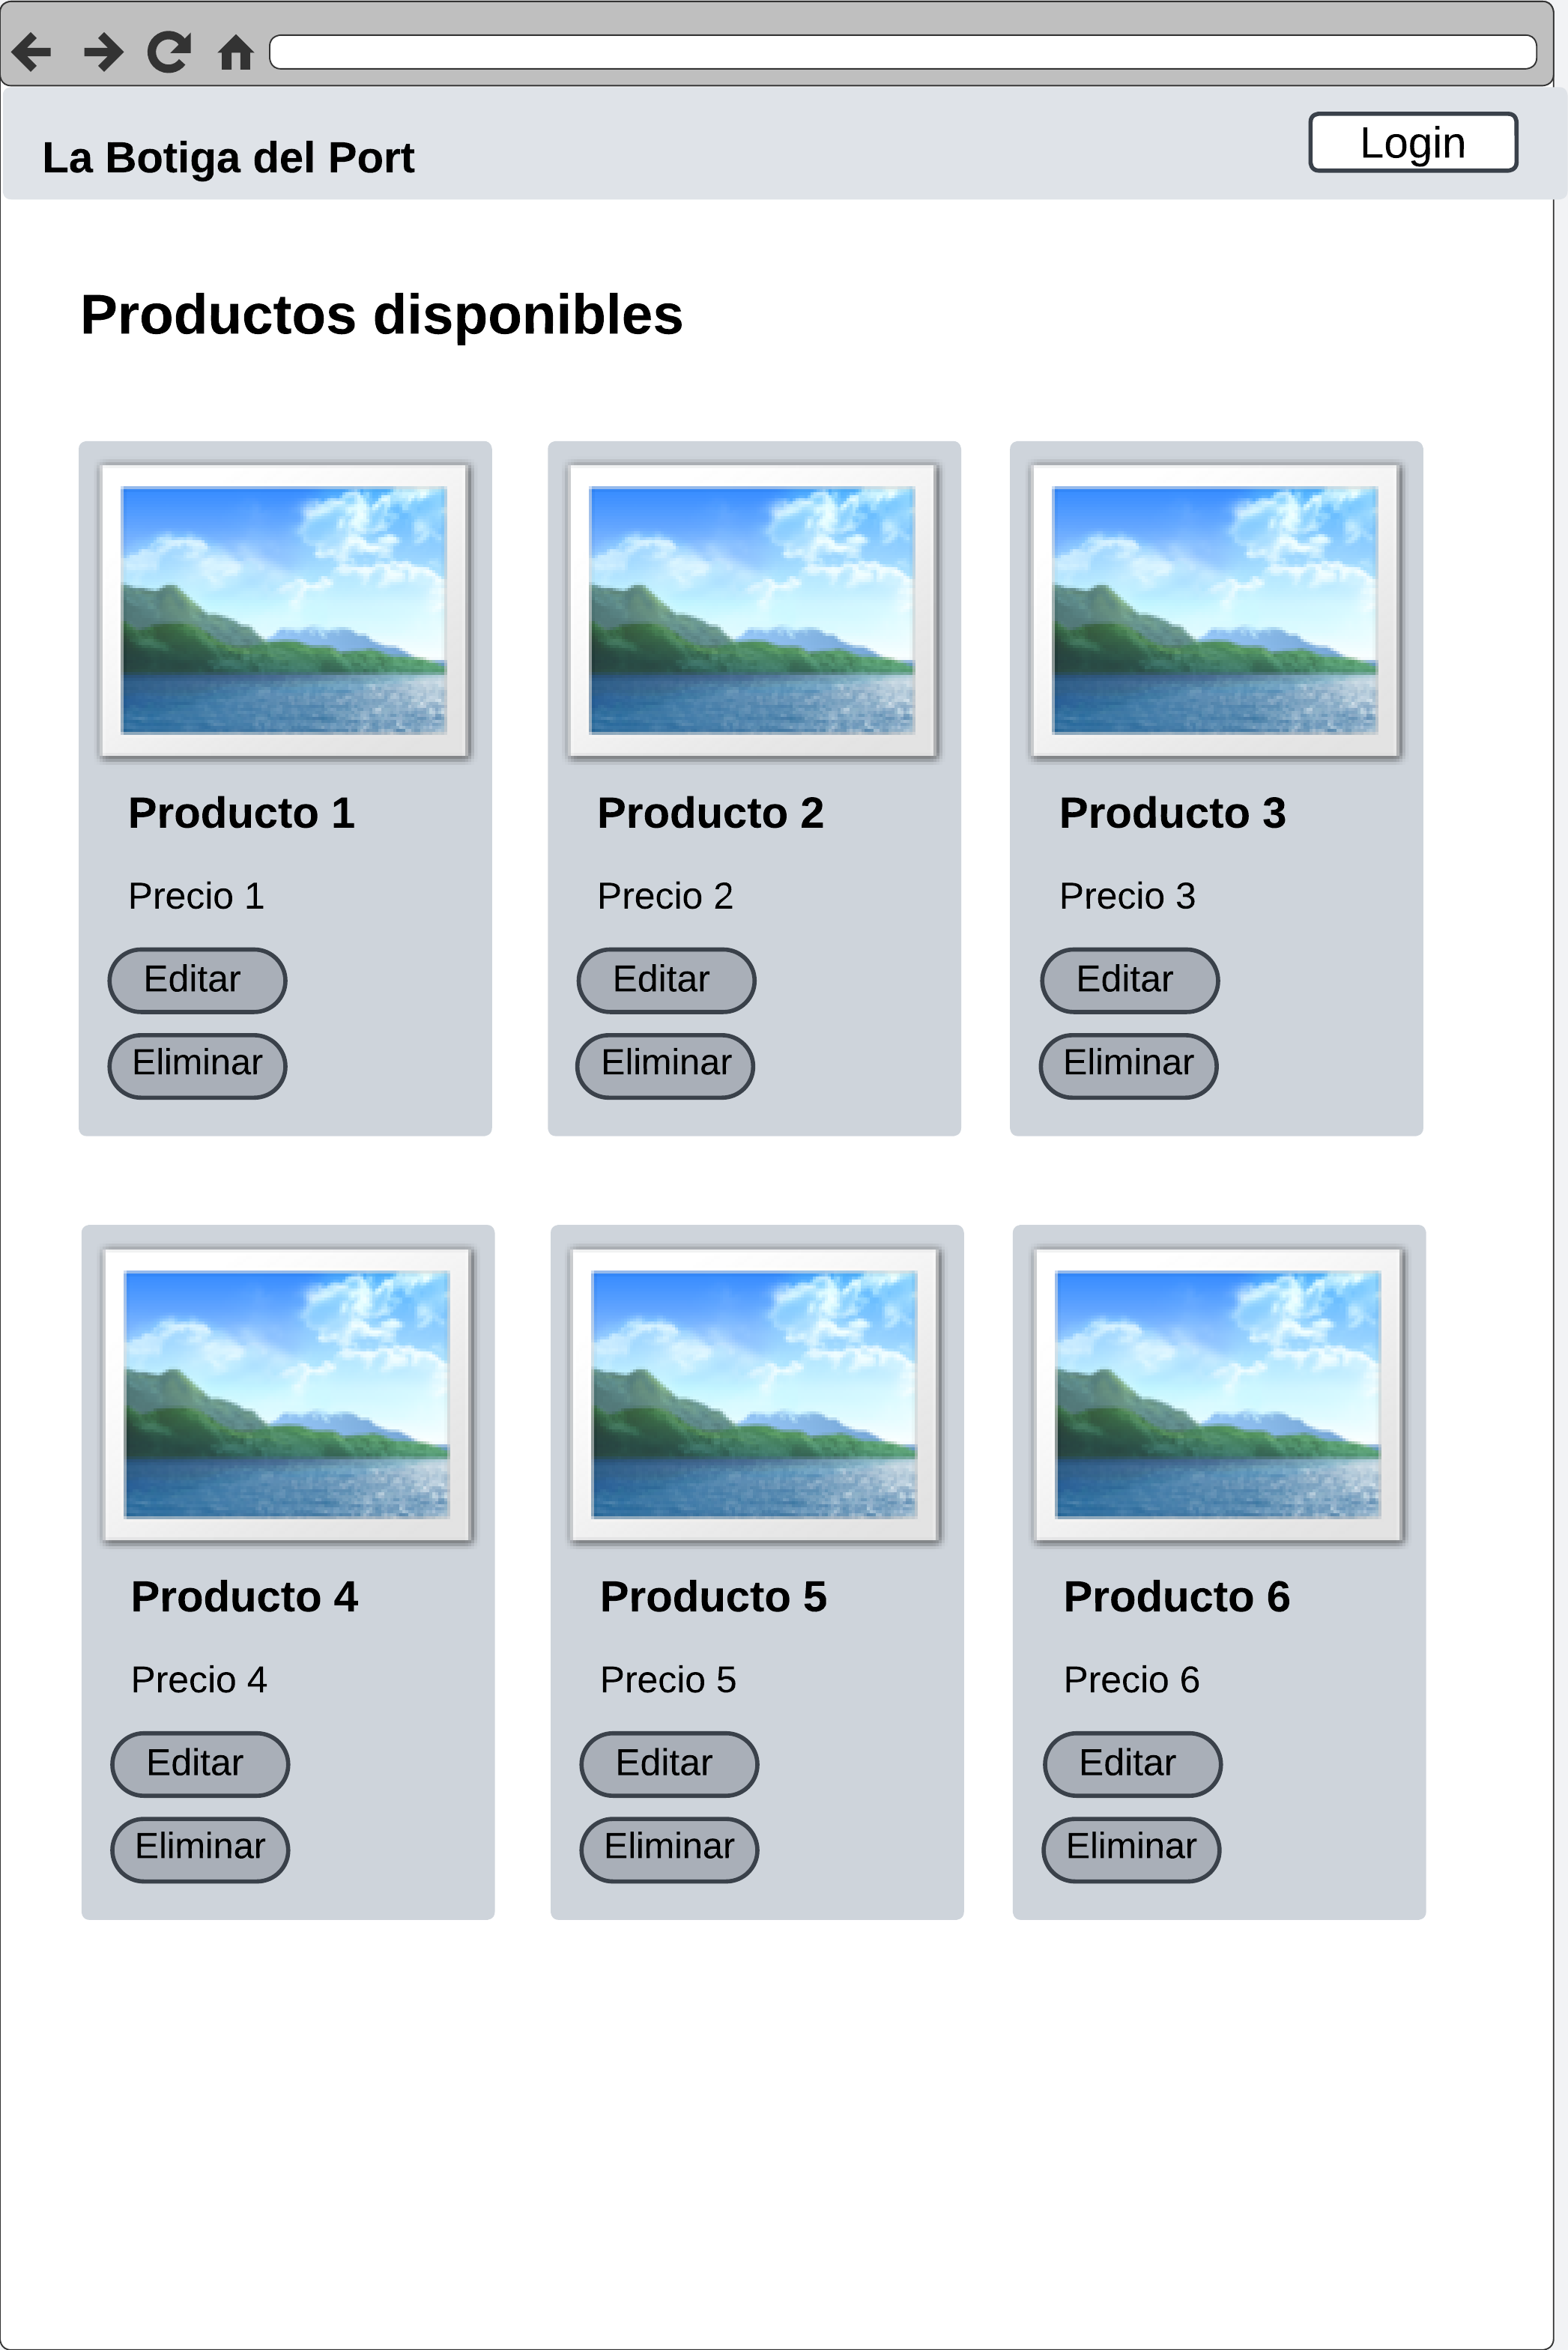
\includegraphics[scale=0.5]{./Images/productos_disponibles.png}
\caption{Modelo de administrador - Productos disponibles.} Fuente: Elaboración propia.

\label{fig:fig9}

\end{center}
\end{figure}

La Figura 4.10 muestra la vista de todas las reservas de cebo efectuadas. Esta interfaz proporciona al administrador una visión general de todas las reservas registradas, junto con opciones para marcarlas como recogidas o eliminarlas según sea necesario.

\begin{figure}[H]
\begin{center}
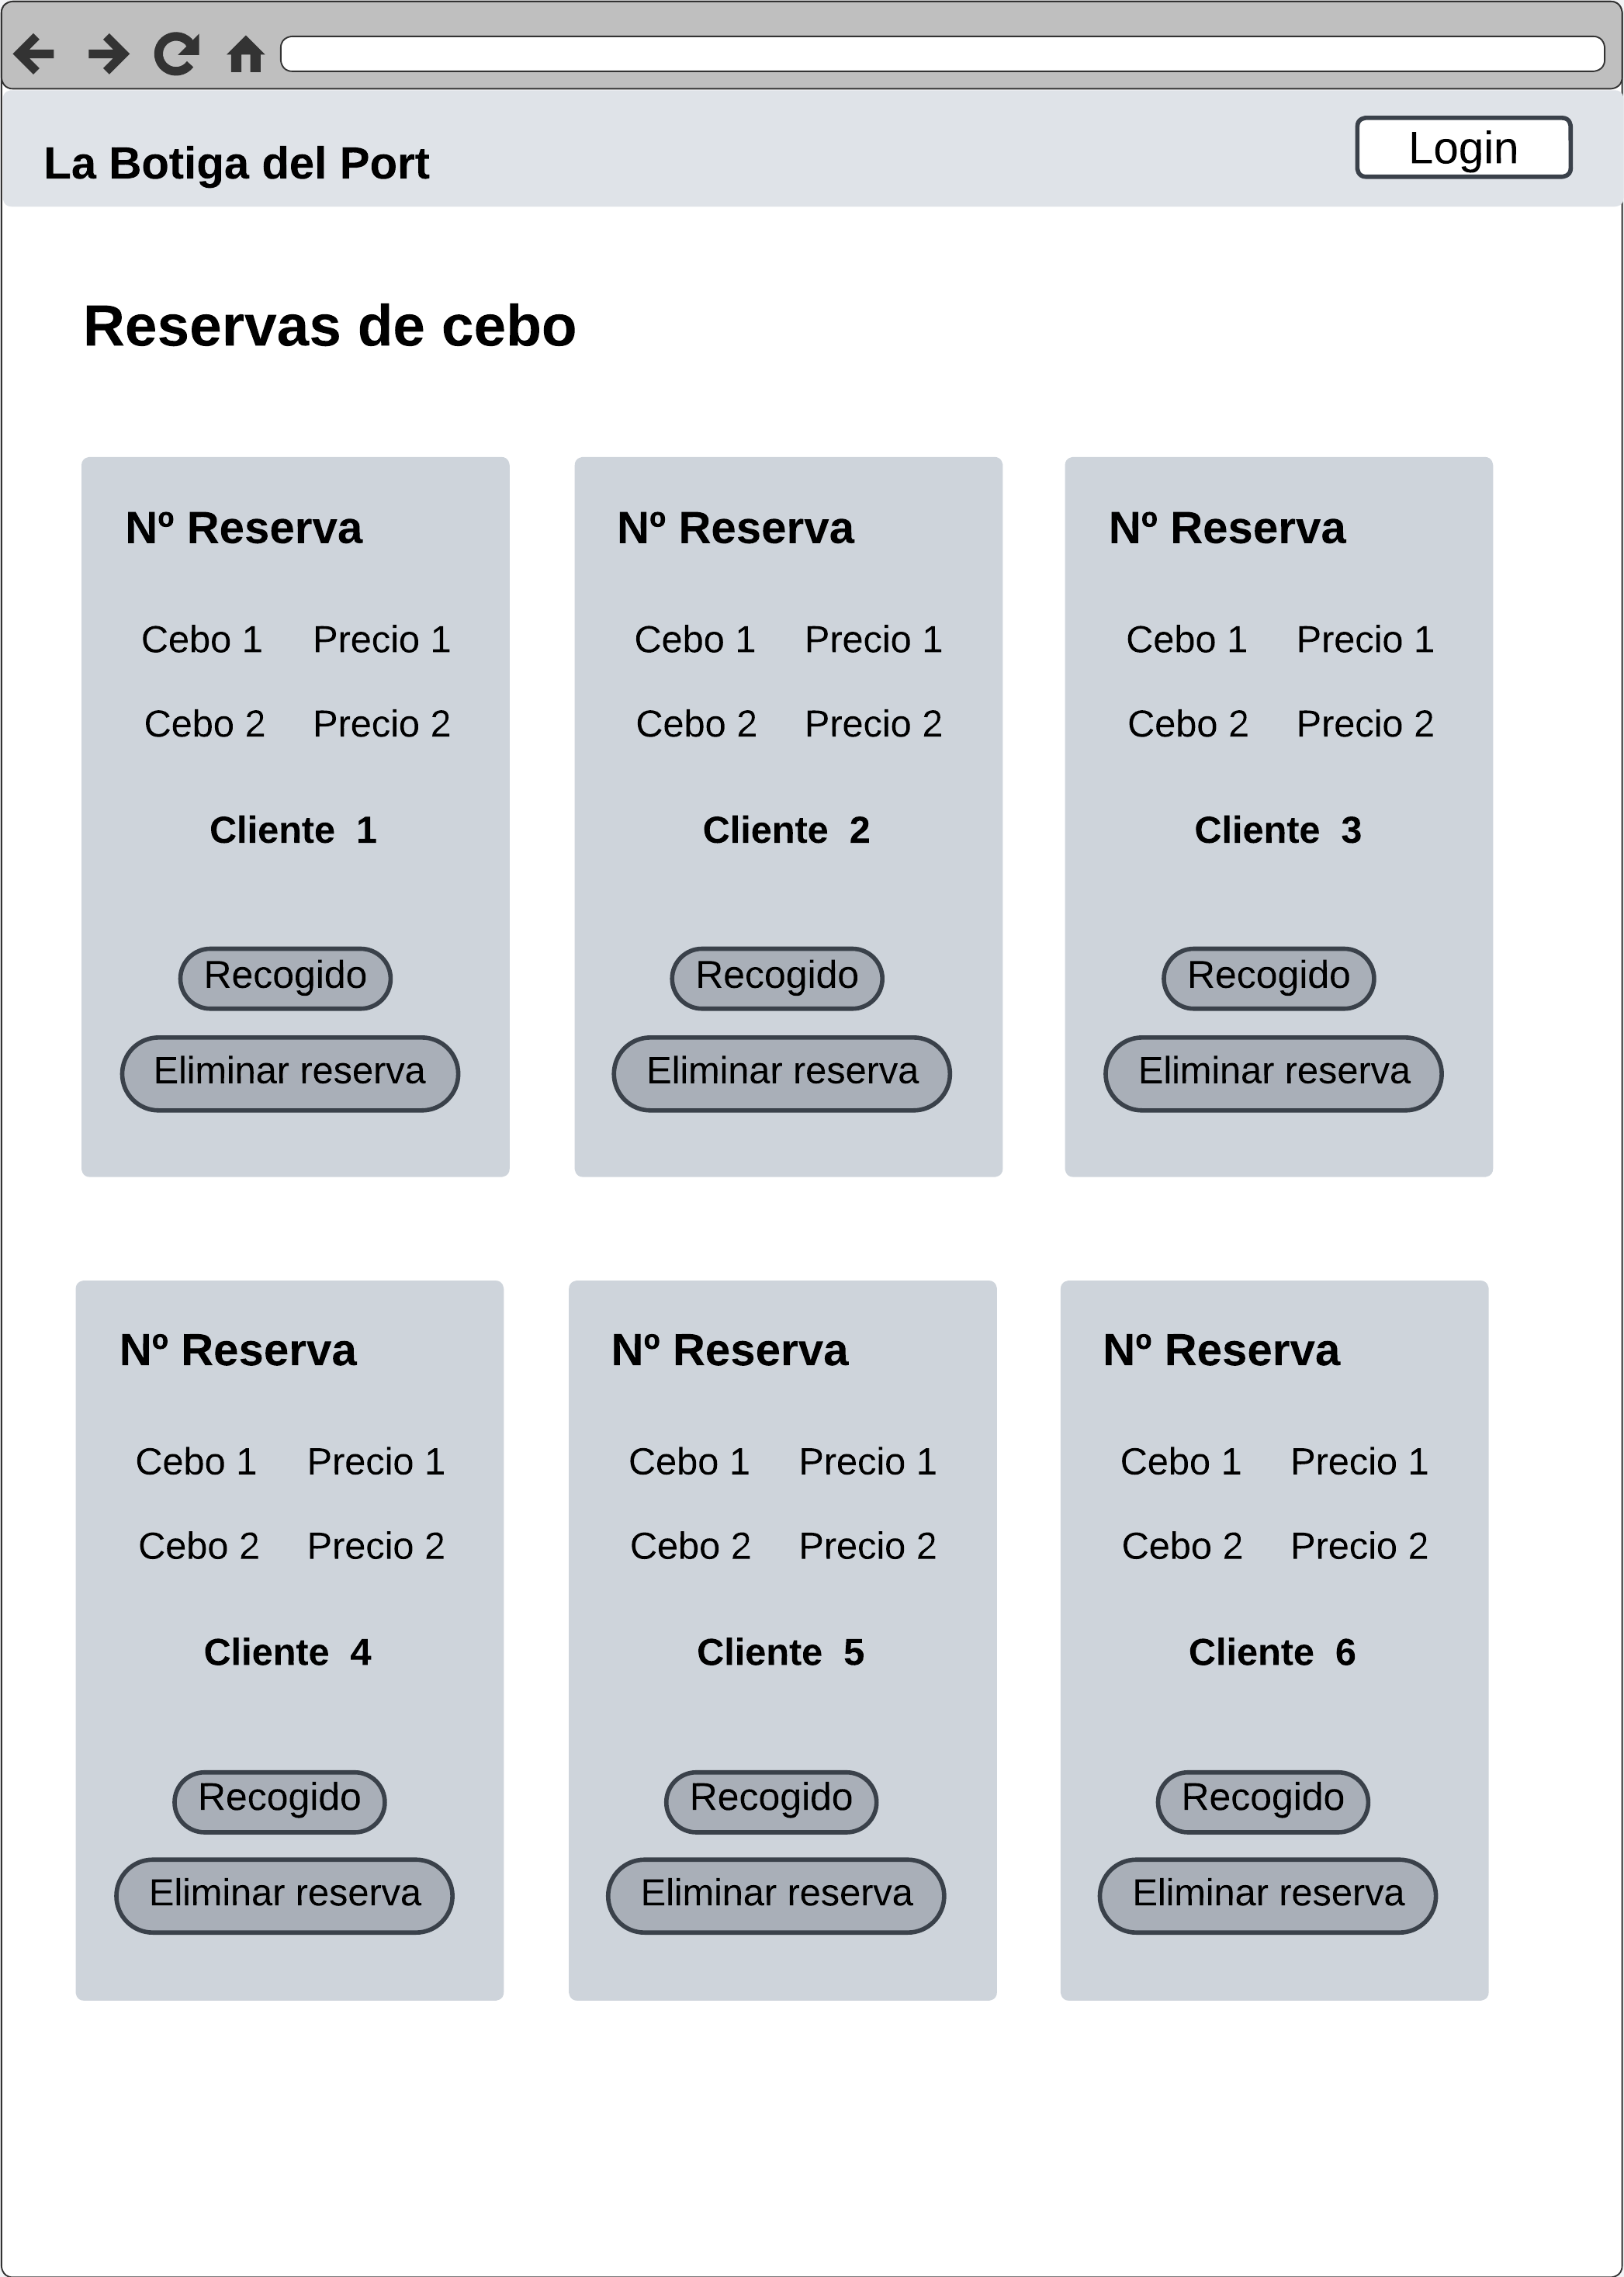
\includegraphics[scale=0.5]{./Images/reserva_cebo_admin.png}
\caption{Modelo de administrador - Reservas de cebo.} Fuente: Elaboración propia.

\label{fig:fig10}

\end{center}
\end{figure}

\section{Diseño BBDD - Diagrama ER}\label{sec:apartado}

La base de datos que sustenta la aplicación ha sido diseñada utilizando un enfoque relacional, con el objetivo de organizar y gestionar de manera eficiente la información generada. A partir de los requisitos específicos de la aplicación, se han identificado las entidades principales, sus atributos relevantes y las relaciones entre ellas. Cada entidad refleja un aspecto clave del sistema, como los productos, usuarios, pedidos y reservas de cebo, mientras que las relaciones aseguran la integridad y coherencia de los datos. Este proceso de modelado ha dado lugar a la creación del diagrama entidad-relación (ER), representado en la \textcolor{naranja}{Figura 4.11}, que proporciona una visión clara y estructurada de cómo se organiza la información en la base de datos y cómo interactúan los distintos elementos entre sí.

\begin{figure}[H]
\begin{center}
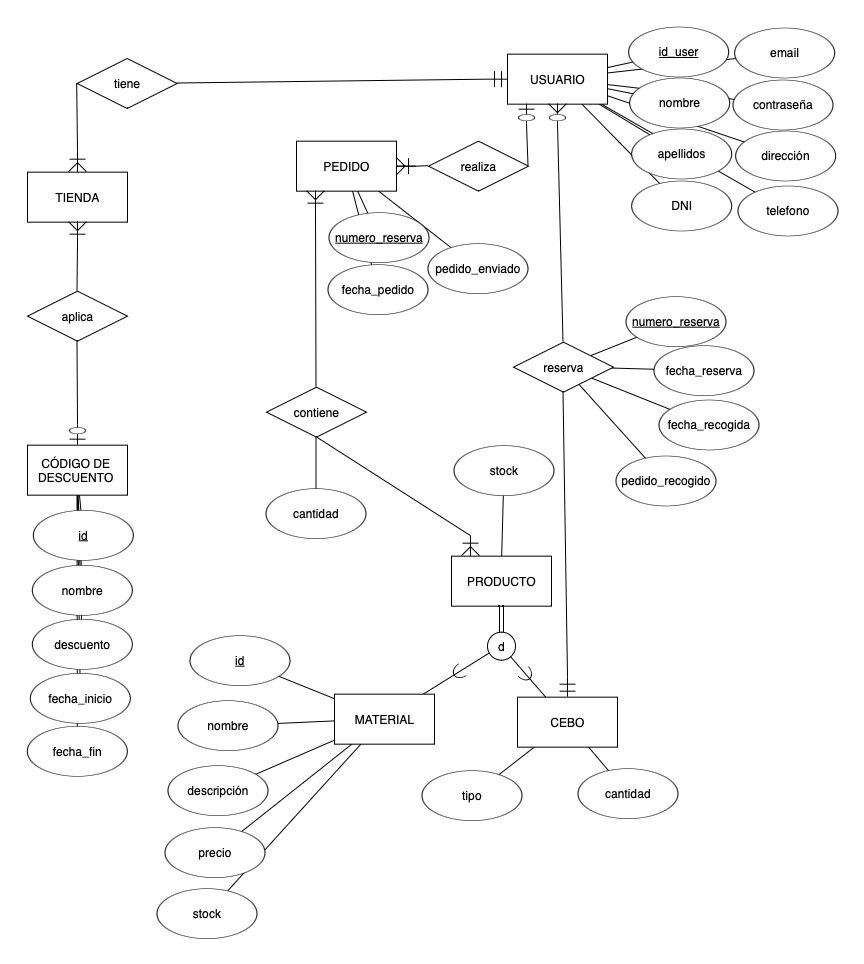
\includegraphics[scale=0.5]{./Images/diagramaER.png}
\caption{Diagrama ER.} Fuente: Elaboración propia.

\label{fig:fig11}

\end{center}
\end{figure}

El diagrama entidad-relación incluye las entidades relacionadas con los usuarios, la gestión de productos, las reservas de cebo y los pedidos, aspectos clave del funcionamiento de la aplicación. También se han incorporado las entidades necesarias para manejar códigos de descuento, los cuales podrán ser aplicados por los usuarios durante el proceso de compra.